\documentclass[
11pt, % The default document font size, options: 10pt, 11pt, 12pt
%oneside, % Two side (alternating margins) for binding by default, uncomment to switch to one side
english, % ngerman for German
singlespacing, % Single line spacing, alternatives: onehalfspacing or doublespacing
%draft, % Uncomment to enable draft mode (no pictures, no links, overfull hboxes indicated)
%nolistspacing, % If the document is onehalfspacing or doublespacing, uncomment this to set spacing in lists to single
%liststotoc, % Uncomment to add the list of figures/tables/etc to the table of contents
%toctotoc, % Uncomment to add the main table of contents to the table of contents
%parskip, % Uncomment to add space between paragraphs
%nohyperref, % Uncomment to not load the hyperref package
headsepline, % Uncomment to get a line under the header
%chapterinoneline, % Uncomment to place the chapter title next to the number on one line
%consistentlayout, % Uncomment to change the layout of the declaration, abstract and acknowledgements pages to match the default layout
]{MastersDoctoralThesis} % The class file specifying the document structure

%%%%%%%%%%%%%%%%%%%%%%%%%%%%%%%%%%%%%%%%%
% Masters/Doctoral Thesis
% LaTeX Template
% Version 3.0 (18/3/22)
%
% This template was downloaded from:
% http://www.LaTeXTemplates.com
%
% Version 2.x major modifications by:
% Vel (vel@latextemplates.com)

% Version 3.x modifications by:
% Felix Friese
%
% This template is based on a template by:
% Steve Gunn (http://users.ecs.soton.ac.uk/srg/softwaretools/document/templates/)
% Sunil Patel (http://www.sunilpatel.co.uk/thesis-template/)
%
% Template license:
% CC BY-NC-SA 3.0 (http://creativecommons.org/licenses/by-nc-sa/3.0/)
%
%%%%%%%%%%%%%%%%%%%%%%%%%%%%%%%%%%%%%%%%%

%----------------------------------------------------------------------------------------
%	PACKAGES AND OTHER DOCUMENT CONFIGURATIONS
%----------------------------------------------------------------------------------------


%\RequirePackage{standalone}
\RequirePackage{sectsty}        % make section heading sans-serif
\RequirePackage{fontawesome5}
\RequirePackage[utf8]{inputenc} % Required for inputting international characters
\RequirePackage[T1]{fontenc} % Output font encoding for international characters
\RequirePackage{mathpazo} % Use the Palatino font by default
\RequirePackage[mathscr]{eucal}
\RequirePackage{microtype}  % somehow make stuff look nicer
\microtypesetup{nopatch=item} % somehow needed
\RequirePackage[backend=bibtex,citestyle=numeric, bibstyle=ieee,natbib=true,sorting=ynt]{biblatex} % Use the bibtex backend
\addbibresource{references.bib} % The filename of the bibliography

\AtEveryBibitem{
    \clearfield{urlyear}
    \clearfield{urlmonth}
    \clearfield{urldate}
}

\RequirePackage{comment}  % comment out sections
% ------------------
% align equations
% ------------------
\RequirePackage{amsmath}  % align equations

%MATHSYMB
\RequirePackage{amssymb}

% ------------------
% wrap figure in text blocks
% ------------------
\RequirePackage{wrapfig}

% ------------------
% fancy plots
% ------------------
\RequirePackage{pgfplots}
\usetikzlibrary{calc, shapes, fit, positioning, arrows.meta, matrix, pgfplots.groupplots}
\usepgfplotslibrary{fillbetween}%, external}
%\tikzexternalize

% use `compat' level 1.3 (or higher) to use the advanced placement features for the axis labels
\pgfplotsset{
    compat=newest
}
% ------------------
% floating stuff, captions and subcaptions, idk
% ------------------
\RequirePackage{float}
\RequirePackage{subcaption}

% ------------------
% very important lorem ipsum package
% ------------------
\RequirePackage{lipsum}

% ------------------
% remark environment
% ------------------
\RequirePackage{amsthm}
\newtheorem*{remark}{Remark}

% ------------------
% code sections
% ------------------
\RequirePackage{fontspec}
\setmonofont{JetBrainsMono}[
Path=./JetbrainsFontFiles/,
Scale=0.85,
Extension = .ttf,
UprightFont=*-Regular,
BoldFont=*-Bold,
ItalicFont=*-Italic,
BoldItalicFont=*-BoldItalic
]
\RequirePackage{minted}



\RequirePackage[autostyle=true]{csquotes} % Required to generate language-dependent quotes in the bibliography



\usemintedstyle{manni}
%----------------------------------------------------------------------------------------
%    COLORS
%----------------------------------------------------------------------------------------
\definecolor{LightGray}{gray}{0.95}
\definecolor{green}{rgb}{0,0.7,0}
\definecolor{modernblue}{HTML}{224fa4}
\definecolor{pyratesdarkred}{HTML}{9f294e}
\definecolor{pyratesgreen}{HTML}{3d734f}
\definecolor{pyratesorange}{HTML}{c76d00}
\definecolor{pyratespurple}{HTML}{473579}


% ------------------
% section number depths
% ------------------
\setcounter{tocdepth}{2}
\setcounter{secnumdepth}{3}

\allsectionsfont{\sffamily}

%----------------------------------------------------------------------------------------
%	MARGIN SETTINGS
%----------------------------------------------------------------------------------------

\geometry{
	paper=a4paper, % Change to letterpaper for US letter
	inner=2.5cm, % Inner margin
	outer=3.8cm, % Outer margin
	bindingoffset=.5cm, % Binding offset
	top=1.5cm, % Top margin
	bottom=1.5cm, % Bottom margin
	%showframe, % Uncomment to show how the type block is set on the page
}

%----------------------------------------------------------------------------------------
%	THESIS INFORMATION
%----------------------------------------------------------------------------------------

% Your thesis title, this is used in the title and abstract, print it elsewhere with \ttitle
\thesistitle{Simulating sedation-induced unconsciousness in a Neural-Mass-Model}
%to improve algorithms for state-of-consciousness detection in patients in the Minimally Conscious State

% Your supervisor's name, this is used in the title page, print it elsewhere with \supname
\supervisor{Dr. Malte \textsc{Schilling}}

% Your examiner's name, this is not currently used anywhere in the template, print it elsewhere with \examname
\examiner{Prof Dr. Helge \textsc{Ritter}}
% Your degree name, this is used in the title page and abstract, print it elsewhere with \degreename
\degree{Master of Science}
% Your name, this is used in the title page and abstract, print it elsewhere with \authorname
\author{Felix \textsc{Friese}}


% Your subject area, this is not currently used anywhere in the template, print it elsewhere with \subjectname
\subject{Intelligent Systems}
% Keywords for your thesis, this is not currently used anywhere in the template, print it elsewhere with \keywordnames
\keywords{EEG, NMM, GABA-A, Propofol, Anaesthesia}
% print it elsewhere with \univname
\university{\href{https://uni-bielefeld.de/}{Bielefeld University}}
% print it elsewhere with \deptname
\department{\href{https://www.uni-bielefeld.de/technische-fakultaet/}{Faculty of Technology}}
% print with \groupname
\group{\href{https://www.uni-bielefeld.de/fakultaeten/technische-fakultaet/forschung/ag-ueberblick/neuroinformatik/}{Neuroinformatics Group}}
%print with \facname
\faculty{\href{https://www.uni-bielefeld.de/technische-fakultaet/}{Faculty of Technology}}

\AtBeginDocument{
\hypersetup{pdftitle=\ttitle} % Set the PDF's title to your title
\hypersetup{pdfauthor=\authorname} % Set the PDF's author to your name
\hypersetup{pdfkeywords=\keywordnames} % Set the PDF's keywords to your keywords
}

\DeclareSIUnit{\molar}{M}

%\usepackage{scrhack}
\RequirePackage{tikz}

\RequirePackage{linegoal}

\RequirePackage{import}
\newcommand\iltodo[1]{
\fcolorbox{orange}{orange!10}{
    \fcolorbox{black}{yellow!70}{\small\faIcon{tasks}~ \texttt{Todo}}
    \hspace{4pt} \texttt{#1}}
}

\newcommand\todo[1]{\par
\noindent\fcolorbox{orange}{orange!10}{\parbox{\linegoal}{
    \fcolorbox{black}{yellow!70}{\small\faIcon{tasks}~ \texttt{Todo}}
    \hspace{4pt} \texttt{#1}}}~\\
}

\newcommand\question[1]{\par
\noindent\fcolorbox{yellow}{yellow!10}{\parbox{\linegoal}{
    \fcolorbox{black}{yellow!70}{\small\faIcon{question}~ \texttt{Question}}
    \hspace{4pt} \texttt{#1}}}~\\
}

\newcommand\incomplete[1]{\par
\noindent\fcolorbox{red}{red!10}{\parbox{\linegoal}{
    \fcolorbox{black}{orange!70}{
        \small\faIcon{exclamation-triangle}~\texttt{Section Incomplete}
    }
\texttt{#1}}}~\\[1em]}


\newcommand{\newremark}[2]{

    \vspace{1em}\par
    \noindent\fcolorbox{yellow}{yellow!10}{
       \begin{minipage}{\linewidth}
        \textbf{Remark} (#1). \textit{ #2 }
       \end{minipage}
    }

    \vspace{1em}\noindent
}

\newcommand{\newremarkimg}[3]{

    \vspace{1em}
    \noindent\fcolorbox{yellow}{yellow!10}{
       \begin{minipage}{\linewidth}
           #2
        \textbf{Remark} (#1). \textit{ #3 }
       \end{minipage}
    }

    \vspace{1em}\noindent
}

\newcommand\citationneeded{\textcolor{blue}{[citation-needed]}}

\begin{document}

\frontmatter % Use roman page numbering style (i, ii, iii, iv...) for the pre-content pages

\pagestyle{plain} % Default to the plain heading style until the thesis style is called for the body content

%----------------------------------------------------------------------------------------
%	TITLE PAGE
%----------------------------------------------------------------------------------------

\begin{titlepage}
\begin{center}

\vspace*{.06\textheight}
{\scshape\LARGE \univname\par}\vspace{1.5cm} % University name
\textsc{\Large Masters Thesis}\\[0.5cm] % Thesis type

\HRule \\[0.4cm] % Horizontal line
{\huge \bfseries \ttitle\par}\vspace{0.4cm} % Thesis title
\HRule \\[1.5cm] % Horizontal line

\begin{minipage}[t]{0.4\textwidth}
\begin{flushleft} \large
\emph{Author:}\\
\href{}{\authorname} % Author name
\end{flushleft}
\end{minipage}
\begin{minipage}[t]{0.4\textwidth}
\begin{flushright} \large
\emph{Supervisor:} \\
\href{https://ni.www.techfak.uni-bielefeld.de/people/mschilli}{\supname} % Supervisor name

\vspace*{.04\textheight}

\emph{Examiner:} \\
\href{https://ni.www.techfak.uni-bielefeld.de/people/helge}{\examname} % Examiner name
\end{flushright}
\end{minipage}\\[3cm]

\vfill

\large \textit{A thesis submitted in fulfillment of the requirements\\ for the degree of \degreename}\\[0.3cm] % University requirement text
\textit{in the}\\[0.4cm]
\groupname\\\deptname\\[2cm] % Research group name and department name

\vfill

{\large \today}\\[4cm] % Date
%\includegraphics{Logo} % University/department logo - uncomment to place it

\vfill
\end{center}
\end{titlepage}

%----------------------------------------------------------------------------------------
%	DECLARATION PAGE
%----------------------------------------------------------------------------------------

% \input{DeclarationPage.tex}


%----------------------------------------------------------------------------------------
%	QUOTATION PAGE
%----------------------------------------------------------------------------------------

% \vspace*{0.2\textheight}

% \noindent\enquote{\itshape
% It is surely important that the differences between coma, deep sleep,
% being under anesthesia, on the one hand, and being alert on the other,
% all involve changes in the brain.}\bigbreak

% \hfill Patricia Churchland

%----------------------------------------------------------------------------------------
%	ABSTRACT PAGE
%----------------------------------------------------------------------------------------

\begin{abstract}
\addchaptertocentry{\abstractname} % Add the abstract to the table of contents
    Understanding the mechanisms behind emergence, modulation and loss of consciousness in the brain
    is still within the bounds of fundamental research.
    Simulation of predictable processes like general anaesthesia in computer models can help to uncover
    which mechanisms play a role in inducing these state-changes.
    Neural-field models have been shown to be able to reproduce the phenomena of drug-hysteresis and
    temporal EEG power-surges during induction and emergence of anaesthesia.
    To find the simplest possible model capable of producing these effects,
    the basic Jansen-Rit model was implemented alongside its subpopulation-extension by David \& Friston.
    Propofol anaesthesia was simulated in both model variants by modulating IPSP decay-time.
    The David-Friston extension was able to reproduce both key phenomena,
    while the basic Jansen-Rit model reproduced the biphasic effect.
    The results substantiate the theory that these effects might be at least partially caused by inherent brain-dynamics
    on population level,
    and further suggest that these dynamics might modulate the preconditions for the emergence of consciousness.
    Additionally, the existence of hysteresis in computer models reinforces the concept of neural inertia.
\end{abstract}

%----------------------------------------------------------------------------------------
%	ACKNOWLEDGEMENTS
%----------------------------------------------------------------------------------------

%\begin{acknowledgements}
%\addchaptertocentry{\acknowledgementname} % Add the acknowledgements to the table of contents
%The acknowledgements and the people to thank go here, don't forget to include your project advisor\ldots
%\end{acknowledgements}

%----------------------------------------------------------------------------------------
%	LIST OF CONTENTS/FIGURES/TABLES PAGES
%----------------------------------------------------------------------------------------
\hypersetup{linkcolor=black}{
    \tableofcontents % Prints the main table of contents
 %   \listoffigures % Prints the list of figures
 %   \listoftables % Prints the list of tables
}
%----------------------------------------------------------------------------------------
%	ABBREVIATIONS
%----------------------------------------------------------------------------------------
\begin{abbreviations}{ll} % Include a list of abbreviations (a table of two columns)

%\textbf{BCI} & \textbf{B}rain \textbf{C}omputer \textbf{I}nterface\\
%\textbf{DoC} & \textbf{D}isorder(s) \textbf{o}f \textbf{C}onsciousness\\
\textbf{EEG} & \textbf{E}lectro\textbf{e}ncephalo\textbf{g}raphy\\
%\textbf{fMRI} & \textbf{f}unctional \textbf{M}agnetic \textbf{R}esonance \textbf{I}maging\\
%\textbf{EIN} & \textbf{E}xcitatory \textbf{I}nter\textbf{n}euron\\
%\textbf{EPSP} & \textbf{E}xcitatory \textbf{P}ost-\textbf{S}ynaptic-\textbf{P}otential\\
\textbf{GA} & \textbf{G}eneral \textbf{A}naesthesia\\
\textbf{GABA} & \textbf{G}amma-\textbf{A}mino\textbf{b}utyric \textbf{A}cid\\
%\textbf{ICA} & \textbf{I}ndependent \textbf{C}omponent \textbf{A}nalysis\\
\textbf{[E/I]IN} & [\textbf{E}xcitatory/\textbf{I}nhibitory] \textbf{I}nter\textbf{n}euron\\
%\textbf{IIN} & \textbf{I}nhibitory \textbf{I}nter\textbf{n}euron\\
%\textbf{IPSP} & \textbf{I}nhibitory \textbf{P}ost-\textbf{S}ynaptic-\textbf{P}otential\\
\textbf{[L/R]OC} & [\textbf{L}oss/\textbf{R}ecovery] \textbf{O}f \textbf{C}onsciousness\\
\textbf{NMM} & \textbf{N}eural \textbf{M}ass \textbf{M}odel\\
\textbf{PC} & \textbf{P}yramidal \textbf{C}ell\\
\textbf{PSD} & \textbf{P}ower \textbf{S}pectral \textbf{D}ensity\\
\textbf{[E/I]PSP} & [\textbf{E}xcitatory/\textbf{I}nhibitory] \textbf{P}ost-\textbf{S}ynaptic-\textbf{P}otential\\
%\textbf{TBI} & \textbf{T}raumatic \textbf{B}rain \textbf{I}njury\\

\end{abbreviations}


%----------------------------------------------------------------------------------------
%	THESIS CONTENT - CHAPTERS
%----------------------------------------------------------------------------------------

\mainmatter % Begin numeric (1,2,3...) page numbering

\pagestyle{thesis} % Return the page headers back to the "thesis" style

% Include the chapters of the thesis as separate files from the Chapters folder

\chapter{Introduction}\label{ch:introduction}

%\section{Initial Motivation}\label{sec:initial-motivation}
%Patients in the Minimally Conscious State can be in more or less conscious states and follow a circadian rhythm,
%with little or no external signs thereof.
%\todo{improve first sentence, cite papers to support it}
%\todo{cite papers with sleep-wake cycle in MCS \cite{cologan_sleep_2013}}
%\todo{cite papers with awareness in MCS}
%
%Lately there have been developments to establish communication channels with these patients by means of BCI-Systems.
%\todo{cite papers with communication in MCS}
%
%To successfully start BCI communication-sessions,
%it is necessary to determine the patients current state of awareness.
%While there are reliable methods to determine consciousness/awareness/wakefulness with healthy subjects,
%\todo{cite papers for EEG sleep/wake detection}
%
%The fact that signals recorded from DoC-patients are structurally different from unimpaired subjects,
%as well as the general difficulty to diagnose an unresponsive patients current state,
%pose a hard challenge.

%Riganello et al. (2021) ''Disorders of Consciousness (DOC) are a spectrum of pathologies affecting one’s ability to
%interact with the external world.
%It can be either due to a traumatic cause [1,2],
%nontraumatic cause [3,4], or a combination of both [5] and gives rise to
%ethically challenging questions [6–8], including the end-of-life decisions.
%For clinical purposes, consciousness is commonly defined by wakefulness (i.e.,
%the presence of spontaneous periods of opening the eyes) and awareness (i.e.,
%the ability for a subject to respond to the internal/external stimuli in an integrated way).
%Two possible conditions of patients with DOC are Unresponsive
%Wakefulness Syndrome/Vegetative State (UWS/VS) [9] and Minimally Conscious State (MCS) [10].
%The first is characterized by a spontaneous opening of the eyes and no sign of
%consciousness but reflexive responses to external stimuli [11,12]; the second condition
%exhibits minimal but discernible signs of non-reflex behaviours which occur
%reproducibly (yet inconsistently) as a response to visual, auditory, tactile, or noxious stimuli.''

%
%- systems for comm with wachkoma
%- problem detecting awareness (VS WAKEFULNESS!)
%- sleep/wake cylces in mcs and vs
\begin{comment}
\section{Motivation}\label{sec:motivation}

%\todo{PK-NMM, COALIA, MENON, LUPPI ->}
%
%NMMs have lately been used to simulate oscillating behavior in anesthesia~\cite{liang_pharmacokinetics-neural_2015,
%    luppi_paths_2021} as
%well as sleep and wake conditions~\cite{bensaid_coalia_2019}.
%Creating and validating realistic models greatly helps the understanding of
%the underlying processes.

Simulating the effects of sedative drugs on the human brain could help
improve our understanding of the complex dynamics of loss and recovery of consciousness.
There are several types of computational models that aim to simulate parts of the brain on different levels of detail.
While models that operate on single-neuron level should in theory be able to reproduce very
realistic brain activity, their scope is oftentimes confined to small areas of the brain. % (computational limits,
Other types of models focus on higher level structures and their interactions, while still being able to reproduce
characteristic higher-level dynamics.
In this thesis we are aiming to reproduce brain-activity in the form of an EEG-like signal,
which, due to the recording method alone, contains only information about higher-level dynamics.
Thus, the model of choice is the widely used Neural-Mass-Model.

The general neuro-chemical [?] effects of the anaesthetic drugs propofol in regard to synaptic receptors are
already well understood and provide a solid starting-point for simulation.

Building on the efforts of Liang et al.~\cite{liang_pharmacokinetics-neural_2015},
who create a model that correlates propofol infusion and resulting effect-site concentration
as well as the NMM proposed by David-Friston ~\cite{david_neural_2003}, a model to simulate a


\todo{BASE EVERYTHING ON PKK-NMM}
first step -> analyse dynamics of system

second step -> correlate to real anaesthesia

\end{comment}

\section{Motivation Deutsch}\label{sec:motivation-deutsch}
Die hochkomplexen Prozesse der Änderung von Bewusstseinszuständen im menschlichen Gehirn sind nach wie vor kaum
verstanden.
Die Definition und Feststellung von Bewusstseinszuständen beruht in der Praxis weiterhin stark auf Verhaltensbasierten
Beobachtungen (e.g. Reiz-Reaktions Tests) \textcolor{blue}{[hier möglicherweise Glasgow Coma Scale erwähnen]}.
Insbesondere bei Menschen die unter traumatischen Hirnschädigungen leiden,
ist diese Herangehensweise jedoch unzureichend, da die Gründe für ausbleibende externe Reaktionen vielseitig sein
können.
Daher werden zunehmend Messungen der Hirnaktivität durch Neuroimaging (fMRT, EEG, \dots) herangezogen um
Bewusstseinszustände
zu bestimmen und zu erforschen, sowie bestimmte Zustandsgrenzen neu zu definieren.
Dabei gibt es bereits beeindruckende Erfolge,
wie beispielsweise eine basale Kommunkation über BCI-Systeme mit Trauma-Patienten die über keinerlei äußerlich
erkennbare Regung als aufmerksam zu erkennen gewesen wären.
Die genauen Mechanismen hinter Zustandsänderungen sowie klare objektive Grenzen zwischen Zuständen sind aber
immer noch der Gegenstand von Grundlagenforschung.
Ein Ansatz um Stück für Stück bessere Einsicht in diese Prozesse zu erlangen, ist die Computer-Simulation von
kontrollierten Zustandsveränderungen, beispielsweise einer Anästhesie, um ein Verständnis für die Veränderung
von Dynamiken der Gehirnaktivtät und deren Auswirkungen zu entwickeln.
Das Betäubungsmittel Propofol wird in der Medizin verwendet um im kontrollierten Rahmen einen völligen
Bewusstseinsverlust zur Durchführung von Operationen herbeizuführen.
Der neurochemische Wirkmechanismus von Propofol auf synaptische Rezeptoren ist bereits gut
erforscht und bietet eine solide Grundlage für die Erforschung von Sedationsprozessen.
Diese Arbeit beschäftigt sich mit der Möglichkeit diese Wirkmechanismen auf Computermodelle von Neuronenpopulationen
im Gehirn anzuwenden und das entstehende Verhalten des Systems zu analysieren sowie Vergleiche zu den
bisherigen neurologischen Erkenntnissen im Bereich Anästhesie zu ziehen.
Ein gängiges Messverfahren um Anästhesie zu beobachten ist das EEG, das insbesondere wegen seines non-invasiven,
portablen und relativ kostengünstigen Einsatzes Verwendung findet.
Als Modell zur Simulation von EEG-ähnlichen Signalen bieten sich sogenannte Neural-Mass-Models (NMMs) an,
die sich auf die Modellierung der Dynamiken von größeren Neuronenpopulationen fokussieren.

%
%\section{Technical Motivation}\label{sec:technical-motivation}
%
%When developing applications that work with live EEG signals and use complex processing steps
%and/or application states,
%it is oftentimes tedious to ensure the application's correct function during development.
%This is due to multiple factors, including potential issues with the recording hardware and the
%complexity of the signal itself.
%Problems that could be caused by faulty implementations as well as the recording setup (producing poor
%signals) are especially hard to pinpoint.
%Long setup times for repeated testing sessions with real subjects further complicate resolving
%any arising issues.
%Therefore, it is very useful to quickly test the implementations with simulated data,
%which can be configured to have specific properties that are relevant to the application, ensuring
%correct function at least under `ideal' conditions.
%While this obviously does not cover the broad variety of issues that will occur in practise,
%it is immensely useful to prevent simple implementation errors and test data-flow and state progression.
%
%Naive approaches to generating EEG-like signals, such as mixing different sinoids and adding gaussian noise,
%work well for testing basic processing steps like artifact- and noise removal,
%bandpass-filtering and signal segmentation.
%However, more sophisticated algorithms, that combine high-level signal features into their reasoning
%and are oftentimes shaped to realistic data, cannot be reliably tested this way.
%
%Even more complications arise, when realistic data for the system's intended use-case is not easily available
%at development time.
%The System mentioned above \todo{actually mention the system} aims to detect the state of consciousness of patients
%with DOC, in order to select appropriate moments for communication.
%Unfortunately, the EEG signals of DOC-patients have fundamentally different characteristics compared to the signals
%recorded from healthy subjects.
%While it is relatively easy to record segments of EEG data from healthy subjects in different states of consciousness
%and label them accordingly, correctly labeled data for patients with DOC is practically unavailable for a number of
%reasons: The obvious challenge of determining the current state of consciousness for a person
%\todo{finish sentence...}

\section{Related Work}\label{sec:related-work}
There have been many efforts to simulate different states of consciousness with NMMs. A particularly sophisticated
example is Bensaid et al.'s COALIA Framework~\cite{bensaid_coalia_2019}, which is able to produce realistic
resting-state EEG-like signals for sleep and wakefulness, by using the output of over 60 interconnected NMMs and
applying a transformation onto scalp electrodes using a realistic head-model with tissue conductivities.
Liang et al.~\cite{liang_pharmacokinetics-neural_2015} focussed on relating propofol-induction to effect-site
concentration, which is an important parameter in any model for anaesthesia-simulation.

\section{Collection of Quotes}

'Although our understanding of the actions of propofol at the molecular level is quite extensive,
we do not entirely understand how these molecular effects translate into alterations in cellular,
synaptic and neural network function, and in turn cause unconsciousness [88].
This knowledge gap is, at least in part, the result of a lack of a generally accepted theory of consciousness.
In recent years, cognitive neuroscience has seen a resurgence of interest in this topic,
with attempts to integrate anaesthesia and sleep research in order to address this deficiency.
This resurgence has revealed several brain areas that play a crucial role in generation of consciousness,
and which are extensively influenced by hypnotic drugs.'
\cite{sahinovic_clinical_2018}\\[1em]



% Chapter Template

\chapter{Background \& Starting Points}\label{ch:theoretical-concepts} % Main chapter title

%
\section{States of Consciousness}

\subsection{Definition}
    \qquad \todo{which states of consciousness are commonly defined}
\subsection{State Transitions}
\subsubsection{Natural Transitions}
    \qquad \qquad \todo{how states transition into each other naturally}
\subsubsection{Sedation}
    \qquad \qquad \todo{how sedation differs from natural loss of consciousness}
\subsection{Disorders of Consciousness}
    \qquad \todo{the symptoms of DOCs}
% \begin{itemize}
%	\item How do we define States of Consciousness?
%	\item What do we know about them (and what do we not)?
%	\begin{itemize}
%		\item How do these states change (naturally)?
%		\item What has an influence on the state?
%		\item What happens for DOCs?
%	\end{itemize}
% \end{itemize}



%\pagebreak
\section{EEG}\label{sec:eeg}

\subsection{Measurement}\label{subsec:measurement}
\qquad \todo{how the EEG is measured technically and which neuronal processes it actually
observes (signal amplification, pyramidal cells, ...)}
\subsection{Advantages/Disadvantages}\label{subsec:advantages/disadvantages}
\qquad \todo{spatial/temporal resolution, invasiveness, ...}
\subsection{States of Consciousness in the EEG Signal}\label{subsec:states-of-consciousness-in-the-eeg-signal}
\qquad \todo{how do the states differ in the signal}
\subsubsection{State Detection in healthy Subjects}
 \qquad \qquad \todo{rough explanation of prevalent algorithms}
\subsubsection{State Detection in Subjects with DOC}
 \qquad \qquad \todo{issues with data collection, structurally different source signal, ...}
\subsection{Simulation}\label{subsec:simulation}

\subsubsection{Motivation}
 \qquad \qquad \todo{what can we hope to achieve by simulating an EEG signal}
\subsubsection{Approaches}
 \qquad \qquad \todo{which tools are at our disposal (naive frequency mixing,
    population models, simulating individual neurons, ...)}
 \subsubsection{Model Choice}
 \qquad \qquad \todo{argue about models => why did we land on NMMs/population models?}
 
% \begin{itemize}
%	\item What does the EEG measure?
%	\item Which advantages and disadvantages come with this measuring method?
%	\item How do different states of consciousness, especially sedation, appear in the EEG signal?
%	\item How can these states be detected automatically?
%	\begin{itemize}
%		\item How well does that work, where does it fail?
%		\begin{itemize}
%			\item Why is automatic detection hard in subjects with DOC?
%		\end{itemize}
%	\end{itemize}
% \end{itemize}
\pagebreak
\newcommand*\circled[2][black]{\tikz[baseline=(char.base)]{
    \node[scale=0.85pt,shape=circle, thin,draw=#1!60, fill=#1!5,inner sep=0.1pt] (char) {#2};}}

\tikzset{
    linedot diameter/.store in=\linedot@diameter,
    linedot diameter=2pt,
    linedot spacing/.store in=\linedot@spacing,
    linedot spacing=16pt,
    linedots/.style={
        line width=\linedot@diameter,
        line cap=round,
        dash pattern=on 0pt off \linedot@spacing,
    }
}


\section{Neural Mass Models}\label{sec:neural-mass-models}

\subsection{The Basic Jansen-Rit Model}\label{subsec:the-jansen-rit-model}

The widely used Jansen-Rit Model~\cite{jansen_neurophysiologically-based_1993, jansen_electroencephalogram_1995},
is based on earlier models by Wilson \& Cowan~\cite{wilson_excitatory_1972},
Lopes da Silva et al.~\cite{lopes_da_silva_model_1974, lopes_da_silva_models_1976} and
Zetterberg et al.~\cite{zetterberg_performance_1978}.
It represents a cortical column in the brain, which is made up of three main components,
each modeling a population of neurons with distinct characteristics.

The basic schema of the model is visualized in Fig.~\ref{fig:Jansen Rit Flowchart}, showing the connections
\begin{wrapfigure}{r}{0.5\textwidth}
    \begin{tikzpicture}[
		roundein/.style={circle, draw=green!60, fill=green!5, very thick, minimum size=11mm},
		roundiin/.style={circle, draw=red!60, fill=red!5, very thick, minimum size=11mm},
		rectp/.style={rectangle, rounded corners=2mm, draw=green!60, fill=green!5, very thick},
		trinode/.style={isosceles triangle, isosceles triangle apex angle=60, very thick, draw=cyan!60, shape border rotate=270, fill=cyan!5,},
		]
        
        \pgfdeclarelayer{bg}
        \pgfsetlayers{bg,main}
        
		%Nodes
		
		\node[trinode]    (PC)        {PC};
		\node[roundein]   (EIN)  [above left= 0.5cm and 2.25cm of PC.center] {EIN};
		\node[roundiin]   (IIN) [above right= 0.5cm and 2.25cm of PC.center] {IIN};
		\node[rectp]   (p) [above left=3cm and 1cm of PC.north] {Ext.};
		\node[below= 0.5cm of PC] (pc_out){};
		\node[above= 0.2cm of EIN.north] (ein_out){};
		\node[above= 0.2cm of IIN.north] (iin_out){};
		%Lines
		\draw[-, red] (IIN.north) -- (iin_out.center){};
		\draw[-, green] (EIN.north) -- (ein_out.center){};
		
		\draw[-{Stealth[scale=1.5]}, red] (iin_out.center) -| (PC.30) node[near end, right, black](output){$\circled[red]{$-$}$};
		\draw[-{Stealth[scale=1.5]}, green] (ein_out.center) -| (PC.155) node[near end, left, black](output){$\circled[green]{$+$}$};
		\draw[-{Stealth[scale=1.5]}, green] (p.east) -| (PC.140) node[pos=0.888, right, black](output){$\circled[green]{$+$}$};
		
		
		\draw[-, green] (PC.south) -- (pc_out.center){};% node[near start, right](output){$\circled{$+$}$};
		
		\draw[-{Stealth[scale=1.5]}, green] (pc_out.center) -| (EIN.south){} node[pos=0.85, right, black](output){$\circled[green]{$+$}$};
		\draw[-{Stealth[scale=1.5]}, green] (pc_out.center) -| (IIN.south){} node[pos=0.85, left, black](output){$\circled[green]{$+$}$};
        
        \begin{pgfonlayer}{bg}
        
        
        \filldraw [fill=darkgray!5,draw=darkgray]
            ($ (EIN.west) + (-0.2,1.7) $)
            rectangle ($ (IIN.east) + (0.2,-3) $);
        \node [above left=1.35cm and 0.2 of EIN.west, anchor=west, text=darkgray]{Cortical Column};
        \end{pgfonlayer}
		
	\end{tikzpicture}
    \caption{\textbf{Basic Schema of the Jansen-Rit Model:} Three populations of neurons}
    \label{fig:Jansen Rit Flowchart}
\end{wrapfigure}
between the main components.
There is a population of Pyramidal Cells which receives input from two populations of inter-neurons,
one of which is excitatory while the other is inhibitory.
Each of the inter-neuron-populations receives the output of the PC population.
Additionally, there is external excitatory input to the PC population from other regions of the brain.

The Block Diagram (Fig.~\ref{fig:Jansen Rit Simple}) shows the individual modules of the model.
A population consists of two types of blocks:
The \textit{PSP-Block} models the behavior of the synapses and neuronal somata.
It can be either excitatory or inhibitory and converts the incoming average pre-synaptic pulse density to
an average post-synaptic membrane potential by convolving it with an
impulse response function ($h_e(t)$ and $h_i(t)$, for excitation and inhibition respectively).
The second block (sometimes called \textit{Potential-To-Rate-Block} after it's functionality)
calculates the populations response to this stimulation, transforming the incoming
average membrane potential back into an average pulse density of action potentials.
It may be roughly viewed as a functional counterpart to the axon hillock by establishing a firing threshold
and is usually implemented by a Sigmoid Function ($Sigm$).
External input from other regions of the brain is represented by $p(t)$.
The Connectivity Constants $C_1$, $C_2$, $C_3$ and $C_4$ are a proportional representation of the
average number of synapses between the populations.
The signal most closely related to the EEG and therefore the variable of interest,
is the summed average membrane potential of the PC population ($y_1(t)-y_2(t)$ in Fig.~\ref{fig:Jansen Rit Simple}).

%\todo{explain neurophysiology why $EEG \approx y_1-y_2$, or reference back to explanation in EEG section}\\[1em]

\begin{figure}[H]
    \centering
    \begin{tikzpicture}[
        pc/.style={draw=black!80},
        ein/.style={draw=black!80},
        iin/.style={draw=black!80},
        pcLabel/.style={font=\small,text=black},
        einLabel/.style={font=\small,text=black},
        iinLabel/.style={font=\small,text=black},
        rectNode/.style={draw=black!80, thick},
        roundNode/.style={circle, draw=black!80, thick},
        ]
	    \input{Chapters/Chapter_02_Technical_Concepts/tikz/jr_simple_block_tikz}
\end{tikzpicture}
    \caption{\textbf{Simple Block Diagram after~\parencite{jansen_electroencephalogram_1995}:}
    It's structure might be somewhat confusing when trying to visualize the biological analogy,
        where each population would have individual afferent PSP-Blocks.
        However, the fact that the two interneuron populations share a single excitatory PSP Block,
        because it produces identical results for both of them (disregarding their individual connectivity factor,
        which is simply applied afterwards), is a computational performance gain,
        thus likely explaining the authors' choice.}
    \label{fig:Jansen Rit Simple}
\end{figure}

\subsubsection{Potential-To-Rate Block}
For a neuron to fire an action potential, its membrane potential needs to surpass a certain threshold.
Since we are modeling not a single neuron but a whole population, we need an operator that can transform
the mean membrane potential that the neurons of the population receive as input into an average firing rate
for the whole population.
While neurons within the population may have individual firing-threshold%TODO:[citation-needed],
it can be assumed due to their sheer number,
that these thresholds are normally distributed around some mean value $v_0$. %TODO:[citation-needed]
An additional assumption that this approach rests on,
is that the number of afferent (i.e.\ incoming) connections to the individual neurons is sufficiently
large to justify the assertion that all neurons receive roughly the same stimulation.
This must be modeled by a monotonically increasing function.
The Potential-To-Rate Block represents this process with a Sigmoid.
After multiple iterations by Zetterberg~\cite{zetterberg_performance_1978},
Lopes da Silva~\cite{lopes_da_silva_models_1976} and others~\cite{van_rotterdam_model_1982},
Jansen and Rit~\cite{jansen_neurophysiologically-based_1993,
    jansen_electroencephalogram_1995} landed on the following equation:
\begin{align}
    Sigm(v) = \frac{2e_0}{1+e^{r(v_0-v)}} \label{eq:SigmJansenRit}
\end{align}
The parameter values (Table~\ref{tab:sigmoid_params}) are empirically
determined~\parencite{jansen_neurophysiologically-based_1993}.
The maximum firing rate the population can achieve is set at $5 Hz$.
A mean membrane potential of $6 mV$ (equal to the populations average firing threshold) elicits half
of the maximum firing rate, while $\frac{0.56}{mV}$ defines the steepness.
The plot in Fig.~\ref{fig:Sigmoid} visualizes these properties.
%TODO: mention refractory period
\begin{table}[H]
    \centering
    \begin{tabular}{ |c|c|c|c| }
        \hline
        \multicolumn{2}{|c|}{Parameter} & Default Value & Unit \\
        \hline
        \hline
        half of maximum firing rate & \(e_0\) & \(2.5\)  & \(Hz\)      \\
        \hline
        average firing threshold    & \(v_0\) & \(6.0\)  & \(mV\)      \\
        \hline
        sigmoidal steepness         & \(r\)   & \(0.56\) & \(mV^{-1}\) \\
        \hline
    \end{tabular}
    \caption{Parameters of the Sigmoid Function}
    \label{tab:sigmoid_params}
\end{table}

\begin{figure}[H]

    \centering
    \pgfplotsset{compat = newest}
    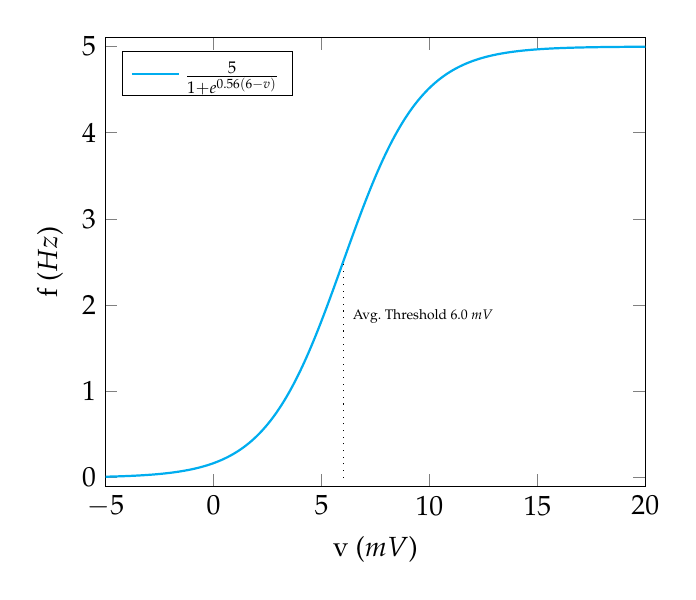
\begin{tikzpicture}
        \begin{axis}
            [
            xmin = -5, xmax = 20,
            ymin = -0.1, ymax = 5.1,
            xlabel = {v ($mV$)},
            ylabel = {f ($Hz$)},
            legend pos=north west,
            legend style={nodes={scale=0.8, transform shape}},
            ],
            \addplot[
                domain = -5:20,
                samples = 200,
                smooth,
                thick,
                cyan,
            ] {5/(1+exp(0.56*(6-x)))};
            \legend{\( \frac{5}{1+e^{0.56(6-v)}} \)}
            \draw [dotted] ([xshift=0.0cm]axis cs:6,0) -- ([yshift=0.0cm]axis cs:6,2.5) node[near end,right,font=\tiny]{
                Avg.\ Threshold 6.0 $mV$};
        \end{axis}
    \end{tikzpicture}
    \caption{Sigmoid (Eq.~\ref{eq:SigmJansenRit}) \parencite{jansen_neurophysiologically-based_1993}} \
    \label{fig:Sigmoid}
\end{figure}

\subsubsection{PSP-Blocks}
%TODO: mention usages of LTI's in Physics, explain this better in general
In Physics, Linear Time-Invariant Systems (LTI systems) are oftentimes used to describe the response of
electrical circuits to arbitrary input signals.
They consist of a kernel function (or impulse-response function),
that models the system's response to a single unit-impulse.
The PSP-Blocks are an LTI system, fully represented by an impulse response function.
It describes a PSP relative to the onset of a pulse.
Since the PSP differs depending on the type of cell (excitatory or inhibitory),
there are two different impulse-response functions.
The parameters for the EPSP (Eq.~\ref{eq:ExcImpResJansenRit}) and IPSP (Eq.~\ref{eq:InhImpResJansenRit})
are given in Table~\ref{tab:psp_params}.
The respective plots are visualized in Fig.~\ref{fig:PSPPlot}.
%TODO: explain how the parameters can be tuned to achieve differnt results, and how that relatates to actual neurobiology
\begin{table}[H]
    \centering
    \begin{tabular}{ |c|c|c|c| }
        \hline
        \multicolumn{2}{|c|}{Parameter} & Default Value & Unit \\
        \hline
        \hline
        Exc. max. amplitude / $e$          & \(A\) & \(3.25\) & \(mV\) \\
        \hline
        %TODO: EXPLAIN 'LUMPED'!!!!
        Lumped repr. of sum of exc. delays & \(a\) & \(100\)  & \(Hz\) \\
        \hline
        Inh. max. amplitude / $e$          & \(B\) & \(22\)   & \(mV\) \\
        \hline
        Lumped repr. of sum of inh. delays & \(b\) & \(50\)   & \(Hz\) \\
        \hline
    \end{tabular}
    \caption{Parameters of the PSP Blocks}
    \label{tab:psp_params}
\end{table}

Excitatory impulse response:
\begin{equation}
    h_e(t) = \begin{cases}
                 Aate^{-at} & \mbox{ } t \geq 0 \\
                 0 & \mbox{ } t < 0
    \end{cases} \label{eq:ExcImpResJansenRit}
\end{equation}

Inhibitory impulse response:
\begin{equation}
    h_i(t) = \begin{cases}
                 Bbte^{-bt} & \mbox{ } t \geq 0 \\
                 0 & \mbox{ } t < 0
    \end{cases} \label{eq:InhImpResJansenRit}
\end{equation}



\begin{figure}[H]
    \centering
    \pgfplotsset{compat = newest}
    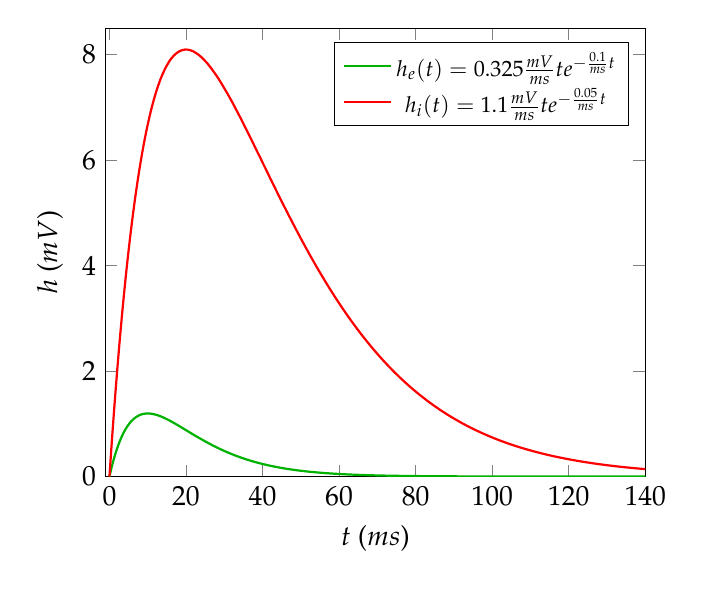
\begin{tikzpicture}
        \begin{axis}
            [
            xmin = -1, xmax = 140,
            ymin = 0, ymax = 8.5,
            xlabel = {$t$ ($ms$)},
            ylabel = {$h$ ($mV$)},
            legend pos=north east,
            legend style={nodes={scale=0.8, transform shape}},
            ],
            \addplot[
                domain = 0:140,
                samples = 200,
                smooth,
                thick,
                green,
            ] {3.25*0.1*x*e^(-0.1*x)};
            \addplot[
                domain = 0:140,
                samples = 200,
                smooth,
                thick,
                red,
            ] {22*0.05*x*e^(-0.05*x)};

            \legend{
                $h_e(t)=0.325\frac{mV}{ms} te^{-\frac{0.1}{ms}t} $,
                $ h_i(t)=1.1\frac{mV}{ms} te^{-\frac{0.05}{ms}t} $
            };

        \end{axis}
    \end{tikzpicture}

    \caption{
        \textbf{Impulse Response Functions:}
        Note the small \textcolor{green}{EPSP}  (Eq.~\ref{eq:ExcImpResJansenRit}) and the
        large \textcolor{red}{IPSP}  (Eq.~\ref{eq:InhImpResJansenRit})~\parencite{jansen_neurophysiologically-based_1993}} \
    \label{fig:PSPPlot}
\end{figure}

Jansen and Rit~\cite{jansen_neurophysiologically-based_1993} justify the difference in amplitude by
referencing Lopes da Silva et al.~\cite{lopes_da_silva_models_1976} and stating that inhibitory neurons
synapse closer to the somata of pyramidal cells (often on the cell body) than excitatory cells,
increasing the effect of an inhibitory neuron about 10-fold.

\todo{maybe go more into detail about the reasons for stronger inhibition}\\[2em]
The output of the Linear System defined by the PSP-Blocks is calculated by a convolution (denoted by $\ast$) of the
incoming impulse density $x(t)$ with the impulse response function $h(t)$ (Eq.~\ref{eq:convolution}).\\
%%%%
% REMARK: CONVOLUTION
%%%%
% \begin{figure}
\begin{wrapfigure}{r}{0.5\textwidth}
    \centering
    \includegraphics[width=0.45\textwidth]{Figures/convolution/wikipedia-citation-needed}
    \caption{\textbf{Convolution:} The area enclosed by $f(\tau)$ and $g(t-\tau)$ is the value of $(f\ast g)(t)$.\\
    \hrulefill \\
    \textit{By Cmglee - Own work, CC BY-SA 3.0  \url{https://commons.wikimedia.org/w/index.php?curid=20206883}}}
    % TODO: RECREATE THIS VISUALIZATION MYSELF
    \label{fig:Convolution}
\end{wrapfigure}
% \end{figure}
%\begin{minipage}{0.6\textwidth}
\begin{remark}[Convolution]
    The convolution of two functions $f(t)$ and $g(t)$ is defined as the integral of their product after one function
    has been reversed and shifted \footnote{There is a very intuitive explanation of
    convolutions by Kalid Azad on his website \url{https://betterexplained.com/articles/intuitive-convolution/}}:
    \[f(t) \ast g(t)= \int_{-\infty}^{+\infty}f(\tau)g(t-\tau) d\tau\]
%     \begin{figure}[H]
%    	\centering
%    		\pgfplotsset{,compat = newest}
%    		\begin{tikzpicture}
%    			\begin{axis}[name=plotf, height=5cm, width=5cm, ticks=none,
%    				xmin = -1, xmax = 120,
%    				ymin = 0, ymax = 9.1,
%    				legend style={nodes={scale=0.5, transform shape}},
%    				legend pos=north east,
%    				],
%    				\addplot[
%    				domain = 0:120,
%    				samples = 200,
%    				smooth,
%    				thick,
%    				green,
%    				] {1.1*x*e^(-0.05*x)};
%    				\legend{$f(\tau)$};
%    			\end{axis}
%    			\begin{axis}[name=plotg, at={($(plotf.east)+(1cm,0)$)}, anchor=west, height=5cm, width=5cm, ticks=none,
%    				legend style={nodes={scale=0.5, transform shape}},
%    				xmin = -120, xmax = 0,
%    				ymin = 0, ymax = 9.1,
%    				legend pos=north east,
%    				],
%    				\addplot[
%    				domain = -120:0,
%    				samples = 200,
%    				smooth,
%    				thick,
%    				red,
%    				] {1.1*(-x)*e^(-0.05*(-x))};
%    				\legend{$g(-\tau)$};
%    			\end{axis}
%
%    			\begin{axis}[name=plotconv1, at={($(plotf.south)-(0,1cm)$)}, anchor=north, height=4cm, width=4cm, ticks=none,
%    				xmin = -120, xmax = 120,
%    				ymin = 0, ymax = 9.1,
%    				%legend pos=north east,
%    				],
%    				\addplot[name path=G,
%    				domain = 0:120,
%    				samples = 100,
%    				smooth,
%    				thick,
%    				green,
%    				] {1.1*x*e^(-0.05*x)};
%    				%\legend{$g(\tau)$};
%    				\addplot[name path=F,
%    				domain = -100:20,
%    				samples = 100,
%    				smooth,
%    				thick,
%    				red,
%    				] {1.1*(-x+20)*e^(-0.05*(-x+20))};
%    				%\legend{$f(\tau)$};
%    				\fill [cyan!20,
%    				intersection segments={
%    					of=F and G,
%    					sequence={R1--L2}
%    				}];
%
%    			\end{axis}
%    		\end{tikzpicture}
%
%    		\caption{Convolution} \
%    		\label{Fig: convolution}
%
%
%     \end{figure}
    If $f(t)$ is a unit-impulse $\delta(t)$ (in our case that would mean each cell of the previous population firing a
    single action potential at the same time) the result is just $g(t)$ (in our case representing a
    single full-amplitude impulse response as the mean membrane potential):
    \[\delta(t) \ast g(t)= \int_{-\infty}^{+\infty}\delta(\tau)g(t-\tau) d\tau = g(t)\]
    In the general case, this process can be used to mathematically model the integration of
    incoming action potential densities in the soma.\\[1em]
    Importantly, the Convolution Theorem states that the convolution of $f(t)$ and $g(t)$ becomes a
    simple multiplication when applying the Laplace Transform:
    \[\mathscr{L}\{f(t) \ast g(t)\}= \mathscr{L}\{f(t)\}\mathscr{L}\{g(t)\} = F(s)G(s)\]
    That means you can calculate a convolution with the inverse Laplace-Transform of the multiplication of
    the functions' individual Laplace-Transforms:
    \[f(t) \ast g(t)= \mathscr{L}^{-1}\{F(s)G(s)\}\]

\end{remark}
% TODO:: USE AND REFERENCE Kalid Azad's Explanation from https://betterexplained.com/articles/intuitive-convolution/
%%%%%%
%\end{minipage}
%\begin{minipage}{0.4\textwidth}

%\end{minipage} \\[1em]
Since the convolution in the time-domain is a computationally heavy operation,
it is oftentimes faster to transform the equation into the Laplace-Domain (see Eq.~\ref{eq:laplace_domain}),
apply the Convolution Theorem and perform the multiplication there,
and transform the results back to the time-domain.
This results in a second order differential equation (Eq.~\ref{eq:sec_ord_nmm}) that
can be efficiently solved by numerical integration.
To obtain this form, we need the Laplace transform $H_e(s)$ (in this context also called \textit{Transfer Function})
of our response function $h_e(t)$:
\[H_e(s) =\mathscr{L}\{h_e(t)\}  = \mathscr{L}\{Aate^{-at} \} = \frac{Aa}{(s+a)^2} = \frac{Aa}{s^2+2as+a^2}\label{eq:laplace_h_e}\]
% \begin{figure}[H]
%	\centering
%	\pgfplotsset{compat = newest}
%	\begin{tikzpicture}
%		\begin{axis}[
%			xmin = -0.07, xmax = 0.05,
%			ymin = -0.1, ymax = 100.0,
%			xlabel = {$t$ ($ms$)},
%			ylabel = {$h$ ($mV$)},
%			legend pos=north east,
%			],
%			\addplot[
%			domain = -0.07:0.05,
%			samples = 200,
%			smooth,
%			thick,
%			red,
%			] {3.25*0.01/((x+0.01)^2)};
%
%			\legend{$H_e(s) = \frac{0.325}{(s+0.01)^2}  $};
%
%		\end{axis}
%	\end{tikzpicture}
%
%	\caption{$H_e(s)$} \
%	\label{Fig: Transfer Function }
% \end{figure}
With that, we can start to transform our initial equation into the desired Second Order System:
\begin{alignat}{5}
    &                                           & &&          \overbrace{y(t)}^{\text{PSP}} \quad &&=& \quad \overbrace{h_e(t)}^{\text{impulse response}} \ast \overbrace{x(t)}^{\text{impulse density}} \label{eq:convolution} \\[1em]
    &                                           & \omit\rlap{applying the Laplace-Transform eliminates the convolution:}                 \nonumber \\[1em]
    &  \stackrel{\mathscr{L}}{\iff} \qquad      & &&                             Y(s) \quad &&=& \quad \overbrace{H_e(s)}^{\text{transfer function}} \cdot X(s)  \label{eq:laplace_domain} \\
    &  \iff                                     & &&                             Y(s) \quad &&=& \quad \frac{AaX(s)}{s^2+2as+a^2}  \nonumber \\
    &  \iff                                     & &&               (s^2+2as+a^2) Y(s) \quad &&=& \quad AaX(s) \nonumber \\
    &  \iff                                     & &&          s^{2}Y(s)+2asY(s)+a^{2}Y(s) \quad &&=& \quad AaX(s) \nonumber \\[1em]
    \omit\rlap{reversing the Laplace-Transform yields a differential equation in the time domain:}     \nonumber \\[1em]
    &  \stackrel{\mathscr{L}^{-1}}{\iff} \qquad & && \ddot{y}(t)+2a\dot{y}(t)+a^{2}y(t) \quad &&=& \quad Aax(t) \nonumber \\
    &  \iff                                     & &&                      \ddot{y}(t) \quad &&=& \quad Aax(t)-2a\dot{y}(t)-a^{2}y(t)  \label{eq:sec_ord_nmm} \\[1em]
    &                                           & \omit\rlap{which can be expressed as a system of two coupled first order equations:}                 \nonumber \\[1em]
    &                                           & &&                       \dot{y}(t) \quad &&=& \quad z(t)  \label{eq:y_t}\\
    &                                           & &&                       \dot{z}(t) \quad &&=& \quad Aax(t)-2az(t)-a^{2}y(t)   \label{eq:z_t}
\end{alignat}

where $y(t)$ is the resulting PSP and $x(t)$ the incoming pulse density.
This works analogously for the inhibitory case with $h_i(t)$.

% \begin{remark}[General Form of Second Order Systems]
%	Comparing (Eq. \ref{eq:sec_ord_nmm}) to the General Form of Second Order Systems (Eq. \ref{eq:gen_sec_order_sys}),
%   we can see that this is a critically damped system ($\zeta = 1$) with gain $K=Aa$ and the natural frequency $\tau$
%   of the system set at $a$.
%	\begin{align}
%		Kf(t) &= \ddot{y}(t)+ 2\zeta \tau\dot{y}(t) + \tau^2y(t) \nonumber \\ 
%		\iff  \ddot{y}(t) &= Kf(t) - 2\zeta \tau\dot{y}(t) - \tau^2y(t)  \label{eq:gen_sec_order_sys}
%	\end{align}
% \end{remark}

%\todo{maybe explain why $\mathscr{L}^{-1}\{sY(s)\} = \dot{y}(t)$ and $\mathscr{L}^{-1}\{s^{2}Y(s)\} = \ddot{y}(t)$}

\subsubsection{Full Linear System}

Taking the two first order equations for $\dot{y}(t)$ (Eq.~\ref{eq:y_t}) and $\dot{z}(t)$ (Eq.~\ref{eq:z_t}),
and the Block diagram (Fig.~\ref{fig:JRBlockColored}) as a base,
we can now state the equations for the full Jansen-Rit Model with it's three populations.
Each PSP-Block $h(t)$ needs it's own system of coupled differential equations.
The value of $x(t)$ can be easily taken from the Block Diagram. $y_0(t)$ is the EPSP received by
both the EIN and IIN population, while $y_1(t)$ is the EPSP and $y_2(t)$ the IPSP received by the PC population:
\begin{equation}
    \begin{aligned}
        \dot{y}_0(t) &= z_0(t) \\
        \dot{z}_0(t) &= \fcolorbox{cyan!80}{cyan!5}{ $ Aa Sigm[y_1(t) - y_2(t)] - 2az_0(t) - a^{2}y_0(t) $}\\
        \dot{y}_1(t) &= z_1(t) \\
        \dot{z}_1(t) &= \fcolorbox{green!80}{green!5}{$ Aa(p(t) + C_{2}Sigm[C_{1}y_0(t)]) - 2az_1(t) - a^{2}y_1(t)$}\\
        \dot{y}_2(t) &= z_2(t) \\
        \dot{z}_2(t) &= \fcolorbox{red!80}{red!5}{$ Bb(C_{4}Sigm[C_{3}y_0(t)]) - 2bz_2(t) -b^{2}y_2(t)$} \\
    \end{aligned}\label{eq:jr_nmm_system}
\end{equation}

\begin{figure}[H]
    \centering
    \begin{tikzpicture}[
        pc/.style={draw=cyan!80, fill=cyan!5},
        ein/.style={draw=green!80, fill=green!5},
        iin/.style={draw=red!80, fill=red!5},
        pcLabel/.style={font=\small,text=cyan!80},
        einLabel/.style={font=\small,text=green!80},
        iinLabel/.style={font=\small,text=red!80},
        rectNode/.style={draw=black!80, thick},
        roundNode/.style={circle, draw=black!80, thick},
        ]
	    \input{Chapters/Chapter_02_Theoretical_Concepts/tikz/jr_simple_block_tikz}
\end{tikzpicture}
    \caption{Colored Block diagram, visualizing the components of (Eq. \ref{eq:jr_nmm_system})}
    \label{fig:JRBlockColored}
\end{figure}

\subsubsection{Connectivity Constants}

A sensible choice for the Connectivity Constants $C_1$ to $C_4$ was determined by Jansen and Rit empirically by
defining a histologically motivated relationship between them ($C = C_1 = \frac{C_2}{0.8} = \frac{C_3}{0.25} =
\frac{C_4}{0.25}$) and varying $C$ until the system produced the desired natural alpha-like activity at $C=C_1=135
\Rightarrow C_2=108; C_3=C_4=33.75$.
Varying $C$ can account for common synaptic phenomena like
neurotransmitter depletion~\parencite{jansen_electroencephalogram_1995}.

\todo{go more into detail about the biological motivation and the effects of these constants on the generated signal}

\subsubsection{Model Input}

The model input $p(t)$ represents the average activity of populations outside the modeled
column that synapse on the columns PC population.
Since this activity's source is so diverse, it is modeled by white noise (120-320 $Hz$).

\todo{go more into detail why the input is modeled like this}
%\begin{wrapfigure}[5]{r}{0.32\textwidth}
\begin{figure}[H]
    \centering
    \pgfplotsset{compat = newest}
    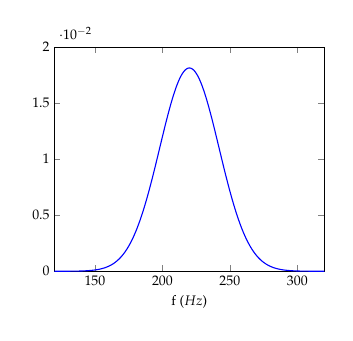
\begin{tikzpicture}[scale=0.5]
        \begin{axis}
            [
            xmin = 120, xmax = 320,
            ymin = 0, ymax = 0.02,
            xlabel = {f ($Hz$)},
            legend pos=outer north east,
            legend style={nodes={scale=1.2, transform shape}},
            ],
            \addplot[
                domain = 120:320,
                samples = 200,
                smooth,
                thick,
                blue,
            ]{(exp(-0.5*((x-220)/22)^2))/(22*sqrt(2*pi))};
            %\legend{$\frac{1}{22\sqrt{2\pi}}e^{-\frac{1}{2}(\frac{x-220}{22})^2}$};

        \end{axis}
    \end{tikzpicture}

    \caption{
        \textbf{Input distribution.}
        The input frequency representing $p(t)$ is sampled from a normal distribution with $\mu=220$ and $\sigma=22$}
    \label{fig:ModelInput}
        %\end{wrapfigure}
\end{figure}

\subsubsection{Model Output}
The simulated data from $y_1-y_2$ while varying $C$ looks like this:
\begin{figure}[H]
    \centering
    \begin{tikzpicture}
        \pgfplotsset{
        %% Axis
            scale only axis,
            width=0.8\linewidth,
            height=2cm,
            every axis/.append style={
                line width=1pt,
                tick style={line width=0.8pt},
                %   grid style={dashed, black!20},
                %  grid=major,
            },
%               %% X-Axis
            xmin=1.0,
            xmax=3,
        }
        \begin{groupplot}
            [
            group style={
                group size=1 by 6,
                vertical sep=2mm,
                xlabels at=edge bottom,
                xticklabels at=edge bottom,
            },
            yticklabel style={
                /pgf/number format/fixed,
                /pgf/number format/precision=2
            },
            legend style={nodes={scale=0.8, transform shape}, thin},
            legend image post style={scale=0},
            xlabel=$t(s)$
            ]
%           \pgfplotsinvokeforeach{0,1,2,3,4,5}{
%             \nextgroupplot
%             \addplot [line width=1pt,solid,color=cyan] table[x=x,y= c#1 ,col sep=comma]{data/test135.csv};
%          }
            \nextgroupplot
            \addplot [line width=1pt,solid] table[x=x,y=c0 ,col sep=comma]{data/simple_c_sweep.csv};
            \legend{$C=68$};
            \nextgroupplot
            \addplot [line width=1pt,solid] table[x=x,y=c1 ,col sep=comma]{data/simple_c_sweep.csv};
            \legend{$C=128$};
            \nextgroupplot
            \addplot [line width=1pt,solid] table[x=x,y=c2 ,col sep=comma]{data/simple_c_sweep.csv};
            \legend{$C=135$};
            \nextgroupplot[ylabel=v ($mV$), every axis y label/.append style={at=(ticklabel cs:1.0)}]
            \addplot [line width=1pt,solid] table[x=x,y=c3 ,col sep=comma]{data/simple_c_sweep.csv};
            \legend{$C=270$};
            \nextgroupplot
            \addplot [line width=1pt,solid] table[x=x,y=c4 ,col sep=comma]{data/simple_c_sweep.csv};
            \legend{$C=675$};
            \nextgroupplot
            \addplot [line width=1pt,solid] table[x=x,y=c5 ,col sep=comma]{data/simple_c_sweep.csv};
            \legend{$C=1350$};

        \end{groupplot}
    \end{tikzpicture}

    \caption{\textbf{Model Output for varying $C$.} Well defined alpha-activity is visible at $C=135$.}
    \label{fig:JansenRitOutput}
\end{figure}

\todo{Explain Graph, generally provide more information to the systems output}

\pagebreak

\subsection{The Sub-Population-Extension by David and Friston}\label{subsec:the-david-and-friston-model}
\incomplete{the whole David-Friston-Section is still very much preliminary}

While the Jansen-Rit model succeeds in generating realistic alpha activity,
real EEG Signals contain much richer spectra~\parencite{steriade_impact_2001}.
David and Friston~\cite{david_neural_2003} proposed a modification to the Jansen-Rit model,
that could produce a more realistic frequency spectrum by introducing sub-populations to the model.
They can be tuned individually to produce oscillations in different frequencies.

\subsubsection{Introducing sub-populations}

David and Friston slightly redefine $h(t)$ by introducing the
parameters $H$ and $\tau$ (see Table~\ref{tab:davidfriston}),
which is just a minor alteration of $A$ and $a$.
\[ h(t)=Aate^{-at} => h(t)=\frac{H}{\tau}te^{-\frac{1}{\tau}} \]
Furthermore, as they are tweaking these parameters to produce slower or faster subpopulations,
they define the products $H_e\tau_e=0.0325mVs$ and $H_i\tau_i=0.44mVs$ as constants.
This is done to preserve the oscillatory behavior of each population~\parencite{david_neural_2003}.
When varying $\tau$, $H$ is therefore adjusted
accordingly ($H_e=\frac{0.0325mVs}{\tau_e}$, $H_i=\frac{0.44mVs}{\tau_i}$).
\begin{table}[H]
    \centering
    \begin{tabular}{ |c|c|c|c|c| }
        \hline
        \multicolumn{2}{|c|}{Parameter} & Value & Unit & Relation to \parencite{jansen_electroencephalogram_1995} \\
        \hline
        \hline
        \rule{0pt}{3ex}Excitatory delays        & \(\tau_e\) & \(0.01\) & $s$  & $ \tau_e = \frac{1}{a} $ \\[1.2ex]
        \hline
        \rule{0pt}{3ex}Inhibitory delays        & \(\tau_i\) & \(0.02\) & $s$  & $ \tau_i = \frac{1}{b} $\\[1.2ex]
        \hline
        \rule{0pt}{3ex}Excitatory synaptic gain & \(H_e\)    & \(3.25\) & $mV$ & $ H_e = A $ \\[1.2ex]
        \hline
        \rule{0pt}{3ex}Inhibitory synaptic gain & \(H_i\)    & \(22\)   & $mV$ & $ H_i = B $ \\[1.2ex]
        \hline
    \end{tabular}
    \caption{Parameters of the PSP Blocks after \parencite{david_neural_2003}}
    \label{tab:davidfriston}
\end{table}
\fcolorbox{red}{red!10}{\parbox{\textwidth}{
    \textbf{Attention:} From now on, the indices $[0,\dots,N]$ for $y$, $h$, $\tau$ and $H$ refer only to
    the subpopulations within a single population.
    The indices used above in the formulation for the Simple Jansen-Rit Model (and the Block Diagram) should not
    be confused with these.
    However, $e$ and $i$ as indices still denote excitatory and inhibitory populations respectively.}} \\[2em]
\begin{figure}[H]
    \begin{tikzpicture}
	\node(sout){};
	\node[shape=rectangle, draw=black, left=0.3cm of sout.center] (SigmPC) {$x(t)$};
	
	\node[shape=rectangle, draw=black, above right=1cm and 2.5cm of sout.center] (H1) {$h_{e_0}(t)$};
	\node[shape=rectangle, draw=black, fill=white, below right=0.2cm and 0.2cm of H1.west] (H2) {$h_{e_1}(t)$};
	\node[shape=rectangle, draw=black, fill=white, below right=2cm and 0.8cm of H2.west] (HN) {$h_{e_N}(t)$};
	\draw[black!80, dots, dot diameter=4pt, dot spacing=25pt, shorten <=8pt, shorten >=8pt] (H2.south) -- (HN.north);
	\node[shape=rectangle, dotted, draw=black, fill=white, fill opacity=0.7, text opacity=1, below right=0.8cm and 0.4cm of H2.west] (Hen) {$h_{e_n}(t)$};
	
	
	\node[left=0.3cm of H1.west](x1){};
	\node[left=0.45cm of H2.west](x2){};
	\node[left=0.85cm of Hen.west](xen){};
	\node[left=1.3cm of HN.west](xN){};
	
	\node[shape=circle, draw=black, right=2cm of H1] (w1) {\small$w_0$};
	\node[shape=circle, draw=black,fill=white, right=2cm of H2] (w2) {\small$w_1$};
	\node[shape=circle, dotted, draw=black, right=2cm of Hen] (wen) {\small$w_n$};
	\node[shape=circle, draw=black, right=2cm of HN] (wN) {\small$w_N$};
	
	
	\node[right=1.1cm of w1.east](y1){};
	\node[right=0.9cm of w2.east](y2){};
	\node[right=0.5cm of wen.east](yen){};
	\node[right=0.001cm of wN.east](yN){};
	
	\node[shape=rectangle, draw=black, right=9cm of sout.center] (pout){$y(t)$};
	
	
	\draw[-] (SigmPC.east) -- (sout.center);
	
	\draw[-] (sout.center) .. controls +(3:1.2) and +(10:-1.5) .. (x1.center);
	\draw[-] (sout.center) .. controls +(3:1.2) and +(10:-1.5) .. (x2.center);
	\draw[-, dotted] (sout.center) .. controls +(3:1.2) and +(10:-1.5) .. (xen.center);
	\draw[-] (sout.center) .. controls +(3:1.2) and +(10:-1.5) .. (xN.center);
	
	
	\draw[->] (x1.center) |- (H1.west);
	\draw[->] (x2.center) |- (H2.west);
	\draw[->, dotted] (xen.center) |- (Hen.west);
	\draw[->] (xN.center) |- (HN.west);
	
	\draw[->] (H1.east) -- (w1.west) node [above, midway]{\tiny$y_0(t)$};
	\draw[->] (H2.east) -- (w2.west)node [above, midway]{\tiny$y_1(t)$};
	\draw[->, dotted] (Hen.east) -- (wen.west)node [above, midway]{\tiny$y_n(t)$};
	\draw[->] (HN.east) -- (wN.west)node [above, midway]{\tiny$y_N(t)$};
	
	
	
	\draw[-] (w1.east) |- (y1.center);
	\draw[-] (w2.east) |- (y2.center);
	\draw[-, dotted] (wen.east) |- (yen.center);
	\draw[-] (wN.east) |- (yN.center);
	
	\draw[->, very thin] (y1.center) .. controls +(3:1.2) and +(10:-1.5) .. (pout.west);
	\draw[->, very thin] (y2.center) .. controls +(3:1.2) and +(10:-1.5) .. (pout.west);
	\draw[->, dotted, thin] (yen.center) .. controls +(3:1.2) and +(10:-1.5) .. (pout.west);
	\draw[->, very thin] (yN.center) .. controls +(3:1.2) and +(10:-1.5) .. (pout.west);
	
\end{tikzpicture}
    \caption{Example of subpopulations ($h_{e_0}(t), \dots, h_{e_N}(t)$) forming an excitatory population $h_e(t)$}
    \label{fig:exc_subpops}
\end{figure}
By introducing subpopulations, we split up the general impulse response function $h(t)$ in $N$ individual
sub-functions:
\[h_n(t) = \frac{H_n}{\tau_n}te^{-\frac{1}{\tau_n}}\] \\[1em]

The previously defined general PSP-Block Equation:
\[y(t)=h(t)\ast x(t)\]
then becomes:
\[y(t)=\sum_{n=0}^{N}{(w_n \cdot h_n(t) \ast x(t))} \hspace{2em}
\text{with}
\hspace{2em} \sum_{n=0}^{N}w_n = 1 \hspace{2em}
\text{and}
\hspace{2em} 0 \leq w_n \leq 1\]
with N individually weighted ($w_n$) and parameterized ($h_n(t)$) subpopulations. \\
We can then declare:
\[y_n(t) = h_n(t) \ast x(t) \quad \text{and} \quad y(t) = \sum_{n=0}^{N} (w_{n}y_n)\]
which produces the following differential equations for a single PSP Block:

\begin{equation}
    \begin{aligned}
        \dot{y}_0(t) &= z_0(t) \\
        \dot{z}_0(t) &= \frac{H_0}{\tau_0} x(t) - \frac{2}{\tau_0}z_0(t) - \left(\frac{1}{\tau_0}\right)^{2}y_0(t)\\
        &\dots\\
        \dot{y}_N(t) &= z_N(t) \\
        \dot{z}_N(t) &= \frac{H_N}{\tau_N} x(t) - \frac{2}{\tau_N}z_N(t) - \left(\frac{1}{\tau_N}\right)^{2}y_N(t)\\
        y(t)         &= w_{0}y_0 + \dots + w_{N}y_N\\
    \end{aligned}\label{eq:davidfriston_subpops}
\end{equation}


%\subsection{möglicherweise auch vorangegangene Paper (Lopez da Silva '76, ...) zur Erklärung heranziehen}


David and Friston further propose an example with two subpopulations for each population with
the following parameters: $\tau_{e_1}=10.8ms$, $\tau_{i_1}=22ms$, $\tau_{e_2}=4.6ms$, $\tau_{i_2}=2.9ms$.
While the kinetics for the first subpopulation were still close
to those of the original populations ($\tau_e=10ms, \tau_i=20ms$, which produce alpha activity),
the second population's parameters were chosen to produce gamma activity.

\todo{put the values in a table}

\begin{figure}[H]
    \centering
    \pgfplotsset{compat = newest}
    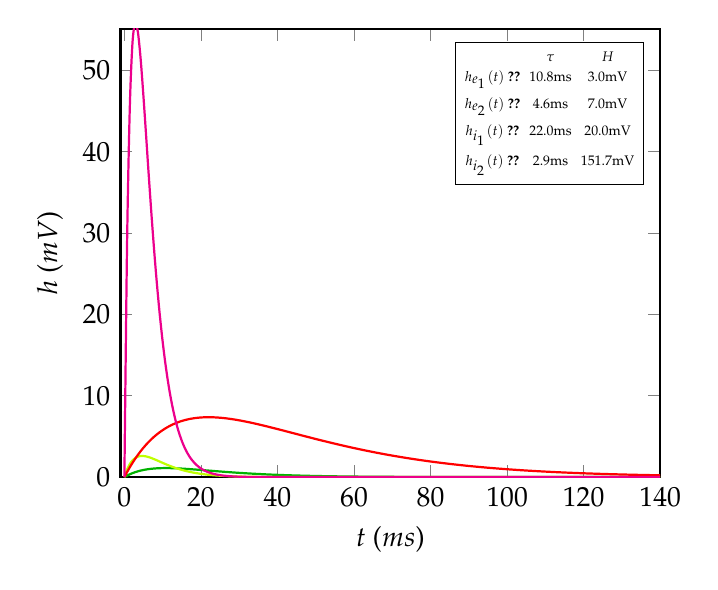
\begin{tikzpicture}
        \begin{axis}
            [
            xmin = -1, xmax = 140,
            ymin = 0, ymax = 55.1,
            xlabel = {$t$ ($ms$)},
            ylabel = {$h$ ($mV$)},
            legend pos=north east,
            legend style={nodes={scale=0.8, transform shape}},
            domain = 0:140,
            samples = 200,
            smooth,
            thick,
            ],
            \addplot[green] {(3.01/10.8)*x*e^(-(1/10.8)*x)};\label{plot:line1}
            \addplot[lime] {(7.07/4.6)*x*e^(-(1/4.6)*x)};\label{plot:line2}
            \addplot[red] {(20/22)*x*e^(-(1/22)*x)};\label{plot:line3}
            \addplot[magenta] {(151.72/2.9)*x*e^(-(1/2.9)*x)};\label{plot:line4}
%
%            \addplot[red, dashed] {(20/22)*x*e^(-(1/22)*x)};\label{plot:line5}
%            \addplot[red, dashed] {(20/24.2)*x*e^(-(1/24.2)*x)};\label{plot:line5.1}
%            \addplot[red, dashed] {(20/26.4)*x*e^(-(1/26.4)*x)};\label{plot:line5.2}
%            \addplot[red, dashed] {(20/28.6)*x*e^(-(1/28.6)*x)};\label{plot:line5.3}
%            \addplot[red, dashed] {(20/30.8)*x*e^(-(1/30.8)*x)};\label{plot:line5.4}
%            \addplot[red, dashed] {(20/33)*x*e^(-(1/33)*x)};\label{plot:line5.5}
%
%            \addplot[magenta, dashed] {(151.72/2.9)*x*e^(-(1/2.9)*x)};\label{plot:line6.1}
%            \addplot[magenta, dashed] {(151.72/3.19)*x*e^(-(1/3.19)*x)};\label{plot:line6.2}
%            \addplot[magenta, dashed] {(151.72/3.48)*x*e^(-(1/3.48)*x)};\label{plot:line6.3}
%            \addplot[magenta, dashed] {(151.72/3.77)*x*e^(-(1/3.77)*x)};\label{plot:line6.4}
%            \addplot[magenta, dashed] {(151.72/4.06)*x*e^(-(1/4.06)*x)};\label{plot:line6.5}
%            \addplot[magenta, dashed] {(151.72/4.35)*x*e^(-(1/4.35)*x)};\label{plot:line6.6}
            \coordinate (legend) at (axis description cs:0.97,0.97);
        \end{axis}
        \tiny
        \matrix [
            draw,
            matrix of nodes,
            anchor=north east,
        ] at (legend) {

            & $\tau$ &    $H$  \\
            $h_{e_1}(t)$~\ref{plot:line1} & 10.8ms &   3.0mV \\
            $h_{e_2}(t)$~\ref{plot:line2} &  4.6ms &   7.0mV \\
            $h_{i_1}(t)$~\ref{plot:line3} & 22.0ms &  20.0mV \\
            $h_{i_2}(t)$~\ref{plot:line4} &  2.9ms & 151.7mV \\
        };
    \end{tikzpicture}

    \caption{\textbf{PSP functions for Subpopulations:}~\ref{plot:line2} and~\ref{plot:line4} are faster
    subpopulations} \
    \label{fig:PSPPlotDavidFriston}
\end{figure}    

\pagebreak
\section{General Anaesthesia}\label{sec:general-anaesthesia}
Having established the theoretical background for our models,
we can approach \ref{goal:implement_propofol} by investigating the effects of propofol in the context of anaesthesia.
GA is usually employed in surgical contexts to keep patients from experiencing pain during medical
procedures, e.g., an operation.
Sedative drugs are carefully administered to the patient by trained practitioners to induce loss of consciousness,
without causing permanent damage to the brain or other parts of the body.
Propofol is the most popular sedative for GA ~\cite{miner_clinical_2007, sahinovic_clinical_2018}
and its effects on the brain have been extensively studied,
which makes it a good candidate for our simulation goals.

\subsubsection{Realistic propofol concentrations during GA}\label{subsubsec:realistic-prop-conc-during-ga}
To estimate sensible parameter ranges for our model,
it is helpful to establish realistic dosages of propofol in clinical practice.
Some works (e.g,~\cite{iwakiri_individual_2005, ferreira_patterns_2020}) state propofol concentrations in $\SI{}{\frac{\micro\gram}{\milli\litre}}$,
while others (e.g.,~\cite{kitamura_effects_2003, mcdougall_propofol_2008}) report values in $\SI{}{\micro\molar}$ (micromolar =
$\SI{}{\frac{\micro\mol}{\litre}}$).
To get comparable numbers, we first need to establish the following relation for propofol
(molar mass: $\SI{178.27}{\gram}$):
\[ \SI{1}{\frac{\micro\gram\hspace{0.5em}\text{\tiny{Propofol}}}{\milli\litre}}  =
\frac{ \SI{1}{\frac{\micro\gram}{\milli\litre}}}{\SI{178.27}{\frac{\gram}{\mol}}} \approxeq \SI{5.609}{\micro\molar} \]
In this work, we will use $\SI{}{\micro\molar}$ as our default unit
but additionally provide original values in $\SI{}{\frac{\micro\gram}{\milli\litre}}$ where they are taken from a source.

Effect-site concentrations ($c_{e}$, concentration near the synaptic receptors) of propofol may easily range
up to $\SI{5}{\frac{\micro\gram}{\milli\litre}} (\approx\SI{28}{\micro\molar})$.
Loss of consciousness (LOC) occurs on average at $c_e \sim\SI{2.0}{\frac{\micro\gram}{\milli\litre}} (\approx\SI{11
.2}{\micro\molar})$,
while the recovery of consciousness (ROC) averages at $c_e \sim\SI{1.8}{\frac{\micro\gram}{\milli\litre}}
(\approx\SI{10.1}{\micro\molar})$.
Both values may vary substantially for individual subjects.
LOC has a strong tendency to occur at higher concentrations than ROC.~\cite{iwakiri_individual_2005,
    ferreira_patterns_2020}
Throughout GA, effect-site concentration is commonly derived from measured
blood-plasma concentration ($c_p$) using more or less complex Pharmacokinetic (PK)-Models
(e.g.,~\cite{eleveld_general_2014, liang_pharmacokinetics-neural_2015}),
as direct measurement of $c_{e}$ in the brain is impractical for obvious reasons.
As our model requires the concentration at the receptors, it will use $c_{e}$ directly, however,
the role of PK-Models with respect to reported effect-site concentrations in many works is crucial
and important to acknowledge.


\subsubsection{Effects of propofol on the inhibitory PSP}
Propofol is a GABA\textsubscript{A} receptor agonist, i.e, it potentiates the effect of inhibitory
GABA neurotransmitters at GABA\textsubscript{A} receptors and thereby modulates
the IPSP~\cite{sahinovic_clinical_2018}.
Research on the effect of propofol on the IPSC (Inhibitory Post-Synaptic Current) and EPSC
of cortical neurons has shown that propofol strongly affects the IPSP decay time.
The EPSP and the amplitude of the IPSP of these neurons are unaffected by propofol.
Effect-site concentrations at clinically relevant levels increase the IPSP decay time
significantly (e.g., around $\SI{10}{\micro\molar}$ the decay time roughly doubles).
\cite{kitamura_effects_2003, mcdougall_propofol_2008}


\subsubsection{Biphasic Effect}\label{subsubsec:biphasic-effect}
A biphasic effect (an initial increase of an effect, that decreases with higher concentrations) in the EEG can be
observed for many sedatives.
At low drug-concentrations during induction (and roughly during loss of consciousness)
there are surges of brain-activity,
which disappear with further increase of the dosage and the onset of the comatose state.
Similar observations have been made during the recovery of consciousness,
when the steadily declining levels of the anaesthetic agent temporarily cause pronounced brain-activity before the
subject fully regains consciousness.
For propofol, a temporary steep increase in EEG amplitude,
loosely correlated with the onset of LOC, as well as ROC can be observed.
\cite{kuizenga_quantitative_1998, kuizenga_biphasic_2001}
% Stage-transition, unstable area between two stable states (consciousness/unconsciousness)


\subsubsection{Hysteresis of propofol}\label{subsubsec:hysteresis}

If the state of a system depends not only on its parameters, but also the systems' history,
this dependency is called hysteresis.
The human body often reacts differently to the same concentration of a drug,
depending on whether the concentration is rising or decaying.
Hysteresis is well documented during propofol-induced GA~\cite{kuizenga_quantitative_1998,
    iwakiri_individual_2005,sepulveda_evidence_2018,ferreira_patterns_2020, su_hysteresis_2020}.
The most prominent effect is a counter-clockwise hysteresis for LOC and ROC (as mentioned
in~\ref{subsubsec:realistic-prop-conc-during-ga});
The loss on responsiveness of subjects usually start at higher concentrations than its return.
While some of that effect might be caused by inaccurate PK-Models,
misgauging the actual effect-site concentration,
there is a growing body of research supporting the notion of neural inertia
(the brain's resistance to state changes)~\cite{su_hysteresis_2020, ferreira_patterns_2020, luppi_inert_2021}.
Nonetheless, doubts remain with respect to the origin
of the observed time-lag~\cite{mckay_pharmacokinetic_pharmacodynamic_2006, sepulveda_evidence_2018}.
% Therories of reasons: - re-initiation more complex than shutdown, phase-transitions

\pagebreak
\section{Effects observed in the Neural-Field-Model by Steyn-Ross}\label{sec:effects-observed-in-the-neural-field-model-by-steyn-ross}
\question{should this section maybe be the FIRST instead of the LAST in this chapter?}
\todo{MAKE THINGS MORE SPECIFIC (frequency ranges, concentrations, etc) WHERE APPLICABLE}
Steyn-Ross et al.\ \cite{steyn_ross_modelling_2004, steyn_ross_sleep_2005, hutt_progress_2011} developed their
model of general anaesthesia based on Liley's\cite{liley_continuum_1999} equations for a mean field model of the cortex.
%\todo{phase-transitions (inherent to the model?)}
They demonstrated that phase-transitions in the model can account for the abrupt change
in brain-state that occurs during induction of anaesthesia~\cite{steyn_ross_modelling_2004}.
The transitions in their model occur due to the existence of multiple stable-states for certain ranges of the
parameters that model the level of anaesthetic agent in the system.
%\todo{biphasic effect}

An interesting finding of their research was the emergence of high-amplitude oscillations during the phase-transitions
of the model.
They correlated this behavior to the `biphasic` effect occurring in general anaesthesia;
at low drug-concentrations during induction (and roughly during loss of consciousness)
there are surges of brain-activity,
which disappear with further increase of the dosage and the onset of the comatose state.
Similar observations have been made during the recovery of consciousness,
when the steadily declining levels of the anaesthetic agent temporarily cause pronounced brain-activity before the
subject fully regains consciousness.
%\todo{hysteresis}

Furthermore, the aforementioned effects are not ``symmetrical'',
meaning the phase-transition on the return path from the ``comatose'' state is not just the reversal of the transition
during induction.
Their model predicts that the transition to the comatose state occurs at higher levels of drug concentration than
the return to the initial state.
Steyn-Ross et al.\ draw parallels to the real effect of drug-hysteresis (see section ~\ref{sec:general-anaesthesia}).
\todo{why do these effects emerge? (partially answered in the beginning of the section, we won't go into mathematical
details like bifurcation analysis here, so i'm not sure yet what to put here...)}
\todo{what can we conclude from the findings?}
These findings are especially intriguing, as the causes of observed hysteresis during induction of general
anaesthesia are yet to be definitively determined~\cite{kuizenga_test_2018, sepulveda_evidence_2018}.
While there is mounting evidence for neural inertia~\cite{ferreira_patterns_2020},
the observed time-lag might be sufficiently explained by pharmacokinetics.
The existence of hysteresis loops in simulated models furthers the theory of neural inertia during loss and recovery
of consciousness.
\todo{can we reproduce these effects with another model?}
As has been stated before, one of the simplest approaches to population based modeling is the Jansen-Rit Model,
which has already been described in detail in section ~\ref{subsec:the-jansen-rit-model}.
Trying to use it as Occam's Razor, it would be interesting to see if it can reproduce the these effects as well.
\todo{improvement idea: `it might be interesting to find the simplest possible model, which we will delve into in the
following section...`}
\pagebreak
%

%----------------------------------------------------------------------------------------
%	UNDERSTANDING THE PSP BLOCK DIFFERENTIAL EQUATIONS
%----------------------------------------------------------------------------------------
\pagebreak
.
\pagebreak
\section{comparision of psp blocks}


\subsection{\parencite{wilson_excitatory_1972}}

\begin{table}[H]
	\centering
	\begin{tabular}{ |c|c|c|c| } 
		\hline
		\multicolumn{2}{|c|}{Parameter}  & Sensible Value & Unit \\
		\hline
		\hline
		prop. of exc. cells firing at $t$ & \(E(t)\) & \( \) & \( \) \\
		\hline
		prop. of inh. cells firing at $t$ & \(I(t)\) & \( \) & \( \) \\
		\hline
		absolute refractory period & $r$ & 4 & $ms$ \\
		\hline
		firing threshold & $\theta$ & & $mV$ \\
		\hline
		propagation delay & $\tau$ & 10 & $ms$ \\
		\hline
		stimulation decay & $\alpha$ & & $mV/s$ (?) \\
		\hline
	\end{tabular}
	\caption{Parameters of \parencite{wilson_excitatory_1972}}
	\label{table:params_wilsoncowan}
\end{table}

Proportion of cells that are excitable at $t$:
\begin{equation}
	1 - \underbrace{\int_{t-r}^{t} E(t') dt'}_{\text{refractory cells}}
\end{equation}

Subpopulation response function (Sigmoid):
\begin{equation}
	\mathscr{S}(x) = \int_{0}^{x(t)} D(\theta) d\theta 
\end{equation}

Excitation in exc. cell
\begin{equation}
	E(t+\tau) = \overbrace{(1 - \underbrace{\int_{t-r}^{t} E(t') dt'}_{\text{refractory cells}}}^{\text{excitable cells}}) \cdot \mathscr{S}_e \cdot \int_{-\infty}^{t}\alpha(t-t') \cdot [C_1E(t') - C_2(I(t') + P(t')] dt'
\end{equation}


\subsection{\parencite{zetterberg_performance_1978} (referencing a model developed in 1973)}

\subsection{\parencite{lopes_da_silva_model_1974}}



\subsection{\parencite{jansen_electroencephalogram_1995}}


\begin{table}[H]
	\centering
	\begin{tabular}{ |c|c|c|c| } 
		\hline
		\multicolumn{2}{|c|}{Parameter}  & Default Value & Unit \\
		\hline
		\hline
		Excitatory synaptic gain & \(A\) & \(3.25\) & \(mV\) \\
		\hline
		Lumped repr. of sum of exc. delays & \(a\) & \(100\) & \(Hz\) \\
		\hline
		Inhibitory synaptic gain & \(B\) & \(22\) & \(mV\) \\
		\hline
		Lumped repr. of sum of inh. delays & \(b\) & \(50\) & \(Hz\) \\
		\hline
	\end{tabular}
	\caption{Parameters of the PSP Blocks2}
	\label{table:psp_params2}
\end{table}

The differential equations for the Second Order System  of this model can be derived by transformations in the Laplace-Domain (see \ref{eq:laplace_domain2}). To obtain the required Transfer-Function, we need the Laplace transform $H_e(s)$ of our response function $h_e(t)$. This is shown in \ref{eq:laplace_h_e2}.


\begin{equation}
	H_e(s) =\mathscr{L}\{h_e(t)\}  = \mathscr{L}\{Aate^{-at} \} = \frac{Aa}{(s+a)^2} = \frac{Aa}{s^2+2as+a^2}\label{eq:laplace_h_e2}
\end{equation}



\begin{alignat}{5}
	&                                           & &&          \overbrace{Y(s)}^{\text{output}} \quad &&=& \quad \overbrace{H_e(s)}^{\text{transfer function}} \overbrace{X(s)}^{\text{input}} \label{eq:laplace_domain2} \\
	&  \iff                                     & &&                             Y(s) \quad &&=& \quad \frac{Aa}{s^2+2as+a^2} X(s) \nonumber \\ 
	&  \iff                                     & &&               (s^2+2as+a^2) Y(s) \quad &&=& \quad AaX(s) \nonumber \\ 
	&  \iff                                     & &&          s^2Y(s)+2asY(s)+a^2Y(s) \quad &&=& \quad AaX(s) \nonumber \\ 
	&  \stackrel{\mathscr{L}^{-1}}{\iff} \qquad & && \ddot{y}(t)+2a\dot{y}(t)+a^2y(t) \quad &&=& \quad Aax(t) \nonumber \\ 
	&  \iff                                     & &&                      \ddot{y}(t) \quad &&=& \quad Aax(t)-2a\dot{y}(t)-a^2y(t)  \label{eq:sec_ord_nmm2} \\[1em]
	&                                           & \omit\rlap{which can be expressed as two first order equations:}                 \nonumber \\[1em]
	&                                           & &&                       \dot{y}(t) \quad &&=& \quad z(t) \nonumber \\ 
	&                                           & &&                       \dot{z}(t) \quad &&=& \quad Aax(t)-2az(t)-a^2y(t) \nonumber 
\end{alignat}

Comparing (\ref{eq:sec_ord_nmm2}) to the General Form of Second Order Systems (\ref{eq:gen_sec_order_sys2}), we can see that this is a critically damped system ($\zeta = 1$) and the natural frequency $\tau$ of the system is set at $a$.

\begin{align}
	f(t) &= \ddot{y}(t)+ 2\zeta \tau\dot{y}(t) + \tau^2y(t) \nonumber \\ 
	\iff  \ddot{y}(t) &= f(t) - 2\zeta \tau\dot{y}(t) - \tau^2y(t)  \label{eq:gen_sec_order_sys2}
\end{align}

\begin{figure}[H]
	\centering
	\includegraphics[width=12cm]{Figures/jansenrit/jansen_rit_ode_graph.png}
	\caption{Simplified Model after \parencite{jansen_electroencephalogram_1995}}
	\label{Fig: Jansen Rit Simple2}
\end{figure}

Taking the two equations for $\dot{y}$ and $\dot{z}$ as a base, we can now state the equations for the full NMM with it's three populations:

\begin{equation}
	\begin{aligned}
		\dot{y}_0(t) &= y_3(t) \\
		\dot{y}_3(t) &= \fcolorbox{green}{white!30}{$ Aa Sigm[y_1(t) - y_2(t)] - 2ay_3(t) - a^2y_0(t) $}\\
		\dot{y}_1(t) &= y_4(t) \\
		\dot{y}_4(t) &= \fcolorbox{red}{white!30}{$ Aa(p(t) + C_2Sigm[C_1y_0(t)]) - 2ay_4(t) - a^2y_1(t)$}\\
		\dot{y}_2(t) &= y_5(t) \\
		\dot{y}_5(t) &= \fcolorbox{blue}{white!30}{$ Bb(C_4Sigm[C_3y_0(t)]) - 2by_5(t) -b^2y_2(t)$} \\
	\end{aligned}
\end{equation}

\begin{equation}
	\begin{aligned}
		\frac{d}{dt}PSP_{EIN} &= PSP_{t_{EIN}} \\
		\frac{d}{dt}PSP_{t_{EIN}} &= \fcolorbox{lime}{white!30}{$ \frac{h_e}{\tau_e}\cdot C_1 Sigm[PSP_{PC}]  -\frac{2}{\tau_e} \cdot PSP_{t_{EIN}} - \left(\frac{1}{\tau_e}\right)^2 \cdot PSP_{EIN} $}\\
		\frac{d}{dt}PSP_{IIN} &= PSP_{t_{IIN}} \\
		\frac{d}{dt}PSP_{t_{IIN}} &= \fcolorbox{teal}{white!30}{$ \frac{h_e}{\tau_e} \cdot C_3 Sigm[PSP_{PC}]  -\frac{2}{\tau_e} \cdot PSP_{t_{IIN}} - \left(\frac{1}{\tau_e}\right)^2 \cdot PSP_{IIN} $}\\
		\frac{d}{dt}PSP_{PCE} &= PSP_{t_{PCE}} \\
		\frac{d}{dt}PSP_{t_{PCE}} &= \fcolorbox{red}{white!30}{$ \frac{h_e}{\tau_e} \cdot (u + C_2 Sigm[PSP_{EIN}])  -\frac{2}{\tau_e} \cdot PSP_{t_{PCE}} - \left(\frac{1}{\tau_e}\right)^2 \cdot PSP_{PCE} $}\\
		\frac{d}{dt}PSP_{PCI} &= PSP_{t_{PCI}} \\
		\frac{d}{dt}PSP_{t_{PCI}} &= \fcolorbox{blue}{white!30}{$ \frac{h_i}{\tau_i} \cdot C_4 Sigm[PSP_{IIN}])  -\frac{2}{\tau_i} \cdot PSP_{t_{PCI}} - \left(\frac{1}{\tau_i}\right)^2 \cdot PSP_{PCI} $}\\
		PSP_{PC} &= PSP_{PCE} - PSP_{PCI}\\
	\end{aligned}
\end{equation}    

\begin{figure}[H]
	\centering
	\includegraphics[width=12cm]{Figures/jansenrit/pyrates_ode_graph.png}
	\caption{Jansen-Rit Model with Modules in PyRates \parencite{gast_pyratespython_2019}}
	\label{Fig: PyratesODE}
\end{figure}

\subsection{\parencite{gast_pyratespython_2019}}
\begin{table}[H]
	\centering
	\begin{tabular}{ |c|c|c|c|c| } 
		\hline
		\multicolumn{2}{|c|}{Parameter}  & Value & Unit & Relation to \parencite{jansen_electroencephalogram_1995} \\
		\hline
		\hline
		\rule{0pt}{3ex}Excitatory delays & \(\tau_e\) & \(0.01\) & $s$ & $ a = \frac{1}{\tau_e} $ \\[1.2ex]
		\hline
		\rule{0pt}{3ex}Inhibitory delays & \(\tau_i\) & \(0.02\) & $s$ & $ b = \frac{1}{\tau_i} $\\[1.2ex]
		\hline
		\rule{0pt}{3ex}Excitatory synaptic gain & \(h_e\) & \(3.25\) & $mV$ & $ A = h_e $ \\[1.2ex]
		\hline
		\rule{0pt}{3ex}Inhibitory synaptic gain & \(h_i\) & \(22\) & $mV$ & $ B = h_i $ \\[1.2ex]
		\hline
		\rule{0pt}{3ex}PSP of $pop$ & \(PSP_{pop}\) &  & & $ PSP_{pop} = y  $ \\[1.2ex]
		\hline
		\rule{0pt}{3ex} Deriv. of PSP of $pop$  & \(PSP_{t_{pop}}\) &  & & $\frac{d}{dt}PSP_{pop} = PSP_{t_{pop}} = z = \dot{y}$ \\[1.2ex]
		\hline
	\end{tabular}
	\caption{Parameters of the PyRates ODEs}
\end{table}


$y_0 = PSP_{PC}, y_1 ~= PSP_{PCE}, y_2 ~= PSP_{PCI}, y_3=?$ 

\begin{equation}
	\begin{aligned}
		\frac{d}{dt}PSP_{EIN} &= PSP_{t_{EIN}} \\
		\frac{d}{dt}PSP_{t_{EIN}} &= \frac{h_e}{\tau_e}\cdot C_1 Sigm[PSP_{PC}]  -\frac{2}{\tau_e} \cdot PSP_{t_{EIN}} - \left(\frac{1}{\tau_e}\right)^2 \cdot PSP_{EIN} \\
		\frac{d}{dt}PSP_{IIN} &= PSP_{t_{IIN}} \\
		\frac{d}{dt}PSP_{t_{IIN}} &= \frac{h_e}{\tau_e} \cdot C_3 Sigm[PSP_{PC}]  -\frac{2}{\tau_e} \cdot PSP_{t_{IIN}} - \left(\frac{1}{\tau_e}\right)^2 \cdot PSP_{IIN}\\
		\frac{d}{dt}PSP_{PCE} &= PSP_{t_{PCE}} \\
		\frac{d}{dt}PSP_{t_{PCE}} &= \fcolorbox{green}{white!30}{$ \frac{h_e}{\tau_e} \cdot (u + C_2 Sigm[PSP_{EIN}])  -\frac{2}{\tau_e} \cdot PSP_{t_{PCE}} - \left(\frac{1}{\tau_e}\right)^2 \cdot PSP_{PCE} $}\\
		\frac{d}{dt}PSP_{PCI} &= PSP_{t_{PCI}} \\
		\frac{d}{dt}PSP_{t_{PCI}} &= \fcolorbox{red}{white!30}{$ \frac{h_i}{\tau_i} \cdot C_4 Sigm[PSP_{IIN}])  -\frac{2}{\tau_i} \cdot PSP_{t_{PCI}} - \left(\frac{1}{\tau_i}\right)^2 \cdot PSP_{PCI} $}\\
		PSP_{PC} &= PSP_{PCE} - PSP_{PCI}\\
	\end{aligned}
\end{equation}                        



\pagebreak
%----------------------------------------------------------------------------------------
%	SECTION 1
%----------------------------------------------------------------------------------------


\section{[TEMP] Neural Mass Models}

Neural Mass Models are computational models of neural populations that aim to simulate population dynamics instead of individual neurons. They operate on the assumption that some of the most studied [frequency-based/state] effects can be modelled by treating a neural population as a single computational unit with one input and one output, representing the sum of all enclosed neuronal activity, thus greatly reducing the computational cost of the model. By combining just a few different populations in a biologically motivated structure, these models can indeed reproduce signals with realistic components. However, when using a model with this degree of simplification, one must always be aware of it's limitations. [citation-needed]

\subsection{History}

\begin{itemize}
	\item \parencite{wilson_excitatory_1972}
	\begin{itemize}
		\item Model for stuff
		\item \( x^n + y^n = z^n \cdot \sqrt{15x} \)
	\end{itemize}
	\item \parencite{lopes_da_silva_model_1974}
	\begin{itemize}
		\item Model for Alpha Activity Generation based on empirically collected physiological parameters 
		\item Histological data of thalamo-cortical relay cells (TCR) and interneurons (IN)
		\item postulated concept: TCR activate inhibitory IN, which inhibt TCRs in return, causing alpha activity
		\item DISTRIBUTED MODEL??
		\item simulation of 144 TCR and 36 IN (ratio based on histological data)
		\item simulation of depolarization and hyperpolarization
		\item Lumped Parameter Model?
		\item TODO: EXPLAIN MATHS!!!!!!!!!!!!!!
	\end{itemize}
	
	\item \parencite{lopes_da_silva_models_1976}
	\begin{itemize}
		\item motivation from freeman (1973) systematic of olfactory system
		\begin{itemize}
			\item groups and layers of with different properties
			\item aggregates: input neurons -> excitatory
			\item populations: groups of neurons with similar properties, input and output (either inhibitory or excitatory)
			\item cartels: interaction of of populations -> feedback loops
			\begin{enumerate}
				\item membrane time constant
				\item length constant
				\item gain factor (strength of interaction), probably most modifiable in terms of neural plasticity
			\end{enumerate}
		\end{itemize}
		\item distributed model (as described in Lds 1974?) "upgraded" to lumped parameter model again
		\
	\end{itemize}
\end{itemize}

\begin{itemize}
	\item \parencite{zetterberg_performance_1978}
	\begin{itemize}
		\item ...
	\end{itemize}
\end{itemize}

\begin{itemize}
	\item \parencite{jansen_neurophysiologically-based_1993-1}
	\begin{itemize}
		\item ...
	\end{itemize}
	\item \parencite{jansen_electroencephalogram_1995}
	\begin{itemize}
		\item ...
	\end{itemize}
\end{itemize}

\begin{itemize}
	\item \parencite{david_neural_2003}
	\begin{itemize}
		\item ...
	\end{itemize}
\end{itemize}

\pagebreak

\subsection{\parencite{jansen_electroencephalogram_1995}}

Jansen and Rit's model is based on the lumped parameter model by \parencite{lopes_da_silva_models_1976}. 
\begin{figure}[htp]
	\centering
	\includegraphics[width=12cm]{Figures/jansenrit/basicmodel.png}
	\caption{Simplified Model after \parencite{jansen_electroencephalogram_1995}}
	\label{Fig: Jansen Rit Simple3}
\end{figure}



\subsection{Disadvantages/Advantages}

While the abstraction that Neural Mass Models provide comes at the price of a degree of reduced biological realism, it enables a more meaningful interpretation of the displayed behavior than a highly complex detailed model that aims to simulate individual neurons and their interactions.[Coombes and Byrne 2019]

%\pagebreak

\chapter{Methodology}\label{ch:methodology}
After establishing the theory required to address our goals,
the next step is the actual implementation of the two models,
the validation of their output (\ref{goal:jr_model},~\ref{goal:df_model}),
and the introduction of a decay-time parameter, which enables modulation of the IPSP (\ref{goal:implement_propofol}).

Instead of implementing the NMMs from scratch,
multiple existing simulation frameworks were considered as a base for this thesis.
The PyRates Framework~\cite{gast_pyratespython_2019} was quickly identified as a flexible and powerful choice
for building custom NMMs.
The following section introduces the PyRates simulation framework
and provides examples of the specific implementation of the JR and DF model.
The implementations are also validated for correctness.
Furthermore, it discusses how the decay-time parameter is added to the implementation.
Lastly, it provides some details on the methodology of analysing the generated data.


\section{PyRates Framework}
\incomplete{The whole PyRates section is still very much preliminary}
The PyRates Framework is a Python software framework, written by Richard Gast and Daniel Rose at the Max-Plank-Institute in Leipzig. It can simulate a wide range of graph-representable neural models, while setting a focus on rate-based population models \parencite{gast_pyratespython_2019}. It wraps computational backends like Numpy and Tensorflow and offers predefined nodes and edges (components that model units like cells or cell populations and the connections between them with mathematical equations) to be used, replaced or extended with custom equations. Furthermore it provides two simple ways to define these components and the derived network configurations: either by YAML-File or within Python code. These configurations are then compiled into optimized executable code with respect to the chosen backend before being executed.
It comes with pre-configured model-definitions for some of the most frequently used models, e.g. the basic Jansen-Rit Circuit \parencite{jansen_electroencephalogram_1995} and the Montbrio-Model \parencite{montbrio_macroscopic_2015}, as well as some variations thereof. It's ease of use, the fact that it could easily reproduce the characteristics of the basic Jansen-Rit model out of the box, and the open-source character made it a sensible choice for this thesis.
\subsection{Network Representations}

\subsubsection{YAML Representation}


\begin{figure}[H]
	\inputminted[frame=lines, linenos, fontsize=\footnotesize, baselinestretch=1.2, bgcolor=LightGray, tabsize=4]
	{yaml}{Chapters/Chapter_02_Technical_Concepts/code/yaml_synapse.yaml}
	
	\caption{Example YAML Synapse}
\end{figure}

\begin{figure}[H]
	\inputminted[frame=lines, linenos, fontsize=\footnotesize, baselinestretch=1.2, bgcolor=LightGray, tabsize=4]
	{yaml}{Chapters/Chapter_02_Technical_Concepts/code/yaml_circuit.yaml}

	\caption{Example YAML Circuit}
\end{figure}
\subsubsection{Python Representation}

\begin{figure}[H]
	\inputminted[mathescape, frame=lines, linenos, fontsize=\footnotesize, baselinestretch=1.2, bgcolor=LightGray, tabsize=4]
	{python3}{Chapters/Chapter_02_Technical_Concepts/code/python_example.py}

	\caption{Python Example for the relevant Operators}
\end{figure}

\subsection{Implementation of the Jansen-Rit Model}
PyRates works with population models by compositing multiple operators, like the PSP- (or Rate-To-Potential-) and Sigmoid- (or Potential-To-Rate) Block into nodes. These nodes represent populations that can then be connected via edges (synapses). For example one might combine two PSP-Blocks (for excitatory and inhibitory input respectively) with a Sigmoid Block to create a PC-Node. This node can then receive rate-input to each of it's PSP-Blocks and  produces rate-output from it's Sigmoid-Block. The EIN- and IIN- nodes are functionally identical and just combine an excitatory PSP-Block with a Sigmoid Block. By connecting these Blocks (see Fig. \ref{fig:pyratesJRBlock}) and adding random input to the excitatory PSP-Block of the PC-Node, the simple Jansen-Rit Circuit is already complete.
\begin{equation}
	\begin{aligned}
		\frac{d}{dt}PSP_{EIN} &= PSP_{t_{EIN}} \\
		\frac{d}{dt}PSP_{t_{EIN}} &= \fcolorbox{pyratesgreen!80}{pyratesgreen!15}{$ \color{pyratesgreen} \frac{H_e}{\tau_e}\cdot C_1 Sigm[PSP_{PC}]  -\frac{2}{\tau_e} \cdot PSP_{t_{EIN}} - \left(\frac{1}{\tau_e}\right)^2 \cdot PSP_{EIN} $}\\
		\frac{d}{dt}PSP_{IIN} &= PSP_{t_{IIN}} \\
		\frac{d}{dt}PSP_{t_{IIN}} &= \fcolorbox{pyratesdarkred!80}{pyratesdarkred!15}{$ \color{pyratesdarkred}\frac{H_e}{\tau_e} \cdot C_3 Sigm[PSP_{PC}]  -\frac{2}{\tau_e} \cdot PSP_{t_{IIN}} - \left(\frac{1}{\tau_e}\right)^2 \cdot PSP_{IIN} $}\\
		\frac{d}{dt}PSP_{PC_E} &= PSP_{t_{PC_E}} \\
		\frac{d}{dt}PSP_{t_{PC_E}} &= \fcolorbox{pyratespurple!80}{pyratespurple!15}{$ \color{pyratespurple}\frac{H_e}{\tau_e} \cdot (p(t) + C_2 Sigm[PSP_{EIN}])  -\frac{2}{\tau_e} \cdot PSP_{t_{PC_E}} - \left(\frac{1}{\tau_e}\right)^2 \cdot PSP_{PC_E} $}\\
		\frac{d}{dt}PSP_{PC_I} &= PSP_{t_{PC_I}} \\
		\frac{d}{dt}PSP_{t_{PC_I}} &= \fcolorbox{pyratesorange!80}{pyratesorange!10}{$ \color{pyratesorange}\frac{H_i}{\tau_i} \cdot C_4 Sigm[PSP_{IIN}])  -\frac{2}{\tau_i} \cdot PSP_{t_{PC_I}} - \left(\frac{1}{\tau_i}\right)^2 \cdot PSP_{PC_I} $}\\
		PSP_{PC} &= PSP_{PC_E} - PSP_{PC_I}\\
	\end{aligned}
\end{equation}    

\begin{figure}[H]
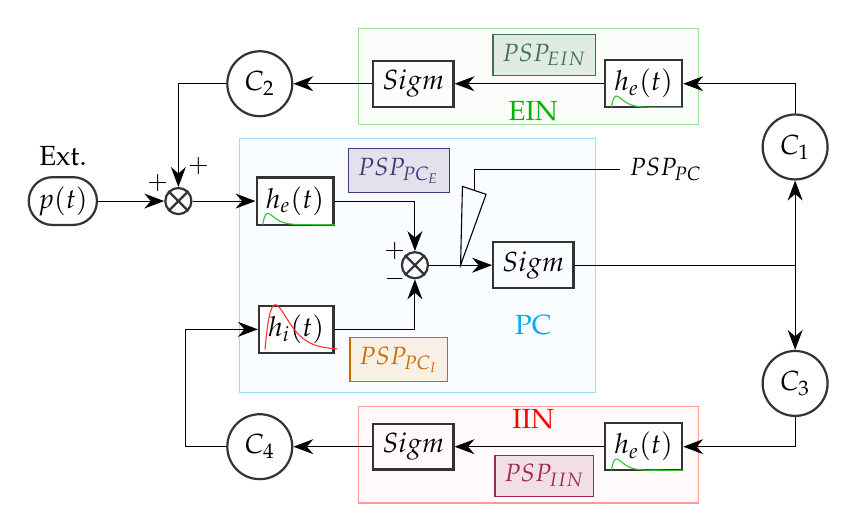
\begin{tikzpicture}[
        pc/.style={draw=cyan!80, fill=cyan!5},
        ein/.style={draw=green!80, fill=green!5},
        iin/.style={draw=red!80, fill=red!5},
        pcLabel/.style={font=\small,text=cyan!80},
        einLabel/.style={font=\small,text=green!80},
        iinLabel/.style={font=\small,text=red!80},
        rectNode/.style={draw=black!80, thick},
        roundNode/.style={circle, draw=black!80, thick},
        ]

\pgfdeclarelayer{bg}
\pgfsetlayers{bg,main}
        
 % Nodes
\node[rectNode] (SigmPC) [] {$Sigm$};
\node[rectNode] (SigmEIN) [above left=2cm and 1cm of SigmPC.center]{$Sigm$};
\node[rectNode] (SigmIIN) [below left=2cm and 1cm of SigmPC.center]{$Sigm$};
\node[rectNode] (PSPPC) [right=1.9cm of SigmEIN.east, fill=white]{$h_e(t)$};
\node[rectNode] (PSPPCI) [right=1.9cm of SigmIIN.east, fill=white]{$h_e(t)$};
\node[rectNode] (PSPEIN) [above left= 0.5cm and 2cm of SigmPC.west, fill=white]{$h_e(t)$};
\node[rectNode] (PSPIIN) [below left= 0.5cm and 2cm of SigmPC.west, fill=white]{$h_i(t)$};
\node[rectNode, rounded corners=3mm] (ext) [left=2cm of PSPEIN.west, label={[]:Ext.}]{$p(t)$};
\node (inpIPSP) [left=0.8cm of PSPIIN.west]{};
\node[roundNode] (c1) [above right=1.2cm and 2.5cm of SigmPC.east]{$C_1$};
\node[roundNode] (c2) [left=1cm of SigmEIN.west]{$C_2$};
\node[roundNode] (c3) [below right=1.2cm and 2.5cm of SigmPC.east]{$C_3$};
\node[roundNode] (c4) [left=1cm of SigmIIN.west]{$C_4$};

% add PC
\node[roundNode] (addPC) [left=0.8cm of SigmPC.west]{};
\draw[-, black!80, thick] (addPC.north west) -- (addPC.south east);
\draw[-, black!80, thick] (addPC.north east) -- (addPC.south west);
% add Excitatory
\node[roundNode] (addExc) [left=0.8cm of PSPEIN.west]{};
\draw[-, black!80, thick] (addExc.north west) -- (addExc.south east);
\draw[-, black!80, thick] (addExc.north east) -- (addExc.south west);

% add PC -> Sigm PC -> PSP PC
\draw[-{Stealth[scale=1.5]}] (addPC.east) -- (SigmPC.west)node[coordinate, pos=0.5](measurepoint){};
\draw[-{Stealth[scale=1.5]}] (SigmPC.east) -| (c1.south);
\draw[-{Stealth[scale=1.5]}] (SigmPC.east) -| (c3.north);


% y0 -> C1 -> Sigm EIN
\draw[-{Stealth[scale=1.5]}] (c1.north) |- (PSPPC.east);
\draw[-{Stealth[scale=1.5]}] (PSPPC.west) -- (SigmEIN.east) node[pos=0.4, above=0.1cm, fill=pyratesgreen!15, draw=pyratesgreen, text=pyratesgreen]{\small$PSP_{EIN}$};

% y0 -> C3 -> Sigm IIN
\draw[-{Stealth[scale=1.5]}] (c3.south) |- (PSPPCI.east);
\draw[-{Stealth[scale=1.5]}] (PSPPCI.west) -- (SigmIIN.east) node[pos=0.4, below=0.1cm, draw=pyratesdarkred, fill=pyratesdarkred!15, text=pyratesdarkred]{\small$PSP_{IIN}$};


% Sigm EIN -> c2 -> add EXC
\draw[-{Stealth[scale=1.5]}] (SigmEIN.west) -- (c2.east);
\draw[-{Stealth[scale=1.5]}] (c2.west) -| (addExc.north) node[pos=0.9, right]{\small$+$};
% external -> add EXC
\draw[-{Stealth[scale=1.5]}] (ext.east) -- (addExc.west) node[pos=0.9, above]{\small$+$};

% add EXC -> PSP EIN
\draw[-{Stealth[scale=1.5]}] (addExc.east) -- (PSPEIN.west);
% PSP EIN -> add PC
\draw[-{Stealth[scale=1.5]}, fill=none] (PSPEIN.east) -| (addPC.north) node[pos=1, left]{\small$+$} node[pos=0.4, above=0.1cm, draw=pyratespurple, fill=pyratespurple!15, text=pyratespurple]{\small$PSP_{PC_E}$};

% Sigm IIN -> C4 -> PSP IIN
\draw[-{Stealth[scale=1.5]}] (SigmIIN.west) -- (c4.east);
\draw[-] (c4.west) -| (inpIPSP.center);
\draw[-{Stealth[scale=1.5]}] (inpIPSP.center) -- (PSPIIN.west);
% PSP IIN -> add PC
\draw[-{Stealth[scale=1.5]}, fill=none] (PSPIIN.east) -| (addPC.south) node[pos=1, left]{\small$-$} node[pos=0.4, below=0.1cm, draw=pyratesorange, fill=pyratesorange!10, text=pyratesorange]{\small$PSP_{PC_I}$};

% electrode
\draw (measurepoint.north) -- (-0.9,1)node[coordinate,pos=0.9](a){} -- (-0.6,0.9)node[coordinate, pos=0.5](b){} -- cycle;
\node (signal)[above right=0.05cm and 2.0cm of a]{\small$PSP_{PC}$};
\draw (b.center) |- (signal.west);


\begin{scope}[shift={(PSPPC.south west)}]
      \begin{axis}[yscale=0.03, xscale=0.16,
            axis x line=none,
            axis y line=none,
            domain=0:140,
            samples=1001,
            xticklabels=\empty,
          ]
          \addplot [green!80] {0.325*x*e^(-0.1*x)};
        \end{axis}
\end{scope}

\begin{scope}[shift={(PSPPCI.south west)}]
      \begin{axis}[yscale=0.03, xscale=0.16,
            axis x line=none,
            axis y line=none,
            domain=0:140,
            samples=1001,
            xticklabels=\empty,
          ]
          \addplot [green!80] {0.325*x*e^(-0.1*x)};
        \end{axis}
\end{scope}

\begin{scope}[shift={(PSPEIN.south west)}]
      \begin{axis}[yscale=0.03, xscale=0.16,
            axis x line=none,
            axis y line=none,
            domain=0:140,
            samples=1001,
            xticklabels=\empty,
          ]
          \addplot [green!80] {0.325*x*e^(-0.1*x)};
        \end{axis}
\end{scope}

\begin{scope}[shift={(PSPIIN.south west)}]
      \begin{axis}[yscale=0.12, xscale=0.16,
            axis x line=none,
            axis y line=none,
            domain=0:140,
            samples=1001,
            xticklabels=\empty,
          ]
          \addplot [red!80] {1.1*x*e^(-0.05*x)};
        \end{axis}
\end{scope}

\begin{pgfonlayer}{bg}
        
    \filldraw [fill=cyan!2,draw=cyan!40]
        ($ (PSPEIN.center) + (-0.7,0.8) $)
        rectangle ($ (PSPIIN.center) + (3.8,-0.8) $);
    \node [below=0.2cm of SigmPC, text=cyan]{PC};
    
    \filldraw [fill=green!2,draw=green!40]
        ($ (SigmEIN.north) + (-0.7,0.4) $)
        rectangle ($ (PSPPC.south) + (0.7,-0.2) $);
    \node [above=1.4cm of SigmPC, text=green]{EIN};
    
    
    \filldraw [fill=red!2,draw=red!40]
        ($ (SigmIIN.north) +  (-0.7,0.2) $)
        rectangle ($ (PSPPCI.south) + (0.7,-0.4) $);
    \node [below=1.4cm of SigmPC, text=red]{IIN};
\end{pgfonlayer}

\end{tikzpicture}
\caption{\textbf{Jansen-Rit Block Diagram as implemented in PyRates:} Each population can be clearly identified by one or more afferent PSP-Blocks and a single Sigmoid that calculates the populations output. This approach is more modular and simplifies conceptual understanding while staying mathematically equivalent. However, due to the explicit fourth PSP-Block it gives up the performance boost.
\quad\todo{possibly the backend-graph-optimization takes care of this? maybe check this later on...} }
\label{fig:pyratesJRBlock}
\end{figure}

\subsection{Implementation of the David \& Friston extensions}


\begin{figure}[H]
	\inputminted[mathescape, frame=lines, linenos, fontsize=\footnotesize, baselinestretch=1.2, bgcolor=LightGray, tabsize=4]
	{python3}{Chapters/Chapter_02_Technical_Concepts/code/psp_subpop.py}
	
	\caption{PSP Block with two Sub-populations in PyRates}
\end{figure}

\subsection{Simulating GABA-A Sedatives}

\quad\todo{why does the reduction of $C$ represent inhibition of the whole system  - what is the difference between thalamic regulation (natural sleep, etc) and GABA-A-receptor binding substances (sedation)? }

\todo{do we have other ways of simulating sedatives in the system?}

\section{Simulating the effects of propofol}\label{sec:simulating-the-effects-of-propofol}


\section{Implementing decay-time modulation}\label{sec:implementing-decay-time-modulation}

To simulate the effects of propofol on the GABA\textsubscript{A}  receptors,
the IPSP (inhibitory response function $h_i$) time-constant $\tau_i$ is increased by a factor
$\lambda$~\cite{hutt_effects_2010}:


\[ h_i(t)=\frac{H_i}{\lambda \cdot \tau_i}te^{-\frac{1}{\lambda \cdot \tau_i}} \]
The effect of increasing $\lambda$ for $h_{i_1}$ and $h_{i_2}$ is visualized in Fig.~\ref{fig:PSPInhibLongPlot}.


\begin{figure}[H]
    \centering
    \pgfplotsset{compat = newest}
    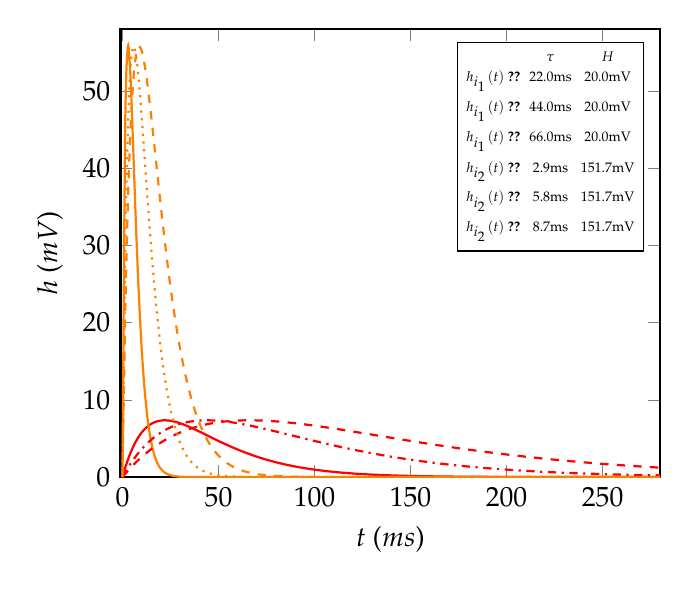
\begin{tikzpicture}
        \begin{axis}
            [
            xmin = -1, xmax = 280,
            ymin = 0, ymax = 58.1,
            xlabel = {$t$ ($ms$)},
            ylabel = {$h$ ($mV$)},
            legend pos=north east,
            legend style={nodes={scale=0.8, transform shape}},
            domain = 0:280,
            samples = 200,
            smooth,
            thick,
            ],
            \addplot[red] {(20/22)*x*e^(-(1/22)*x)};\label{plot:psp3}
            \addplot[orange] {(151.72/2.9)*x*e^(-(1/2.9)*x)};\label{plot:psp4}
            \addplot[red, dash dot] {(20/44)*x*e^(-(1/44)*x)};\label{plot:psp5.10}
            \addplot[red, dashed] {(20/66)*x*e^(-(1/66)*x)};\label{plot:psp5.15}

            \addplot[orange, dotted]{(151.72/5.8)*x*e^(-(1/5.8)*x)};\label{plot:psp6.10}
            \addplot[orange, dashed] {(151.72/8.7)*x*e^(-(1/8.7)*x)};\label{plot:psp6.15}
            \coordinate (legend) at (axis description cs:0.97,0.97);
        \end{axis}
        \tiny
        \matrix [
            draw,
            matrix of nodes,
            anchor=north east,
        ] at (legend) {

            & $\tau$ &    $H$  \\
            $h_{i_1}(t)$~\ref{plot:psp3} & 22.0ms &  20.0mV \\
            $h_{i_1}(t)$~\ref{plot:psp5.10} & 44.0ms &  20.0mV \\
            $h_{i_1}(t)$~\ref{plot:psp5.15} & 66.0ms &  20.0mV \\
            $h_{i_2}(t)$~\ref{plot:psp4} &  2.9ms & 151.7mV \\
            $h_{i_2}(t)$~\ref{plot:psp6.10} &  5.8ms & 151.7mV \\
            $h_{i_2}(t)$~\ref{plot:psp6.15} &  8.7ms & 151.7mV \\
        };
    \end{tikzpicture}

    \caption{\textbf{Inhibitory PSP functions with varying $\lambda$:} \\
        The duration of the effect increases while the amplitude stays
        constant, effectively increasing the charge transfer. ($\lambda$ in [1.0 (no drug-effect, solid lines),
        2.0 (dotted), 3.0 (dashed)])
    }
    \label{fig:PSPInhibLongPlot}
\end{figure}
Varying $\lambda$ between $1$ ($\SI{0}{\micro\molar}$) and $3.0$ ($\sim\SI{30}{\micro\molar}$) appears to be a
sensible choice for the clinically relevant range, given Fig.~\ref{fig:lambda_fit}.

\chapter{Results}\label{ch:results}

\todo{name goals of simulation}
\todo{explain reasoning behind linea increase (close to realistic sedation, but focus on structural exploration of the
possible values)}
% phasendiagram

%propofol-region/vs nicht propofol region
%yapunov kooefizienten, fractale dimension der attraktoren
%chaotische regionen -> welche dimensionen werden ``gedehnt'' oder ``gestaucht''


% hypothese -> dynamische rahmenbedingen, analyse können bewusstsein nicht erfassen, aber notwendige rahmenbedingungen

% muster in wechsel zwischen rahmenbedingungen erkennen

%

%
%\section{The finally used model}\label{sec:the-finally-used-model}
%
%\begin{figure}[H]
%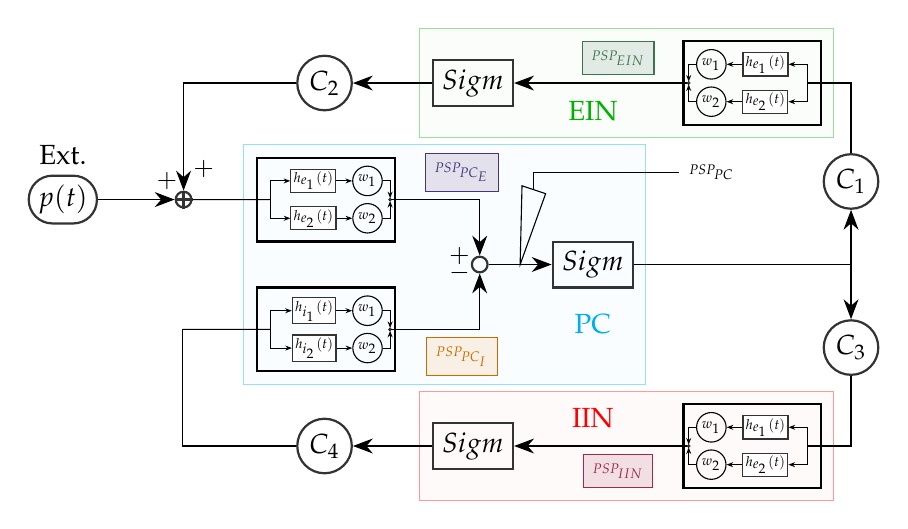
\begin{tikzpicture}[
        pc/.style={draw=cyan!80, fill=cyan!5},
        ein/.style={draw=green!80, fill=green!5},
        iin/.style={draw=red!80, fill=red!5},
        pcLabel/.style={font=\small,text=cyan!80},
        einLabel/.style={font=\small,text=green!80},
        iinLabel/.style={font=\small,text=red!80},
        rectNode/.style={draw=black!80, thick},
        roundNode/.style={circle, inner sep=2pt, draw=black!80, thick},
        ]

\pgfdeclarelayer{bg}
\pgfsetlayers{bg,main}
        
 % Nodes
\node[rectNode] (SigmPC) [] {$Sigm$};
\node[rectNode] (SigmEIN) [above left=2cm and 1cm of SigmPC.center]{$Sigm$};
\node[rectNode] (SigmIIN) [below left=2cm and 1cm of SigmPC.center]{$Sigm$};


%% SUBPOPULATIONS FOR EIN
\node[circle, inner sep=1pt, draw, scale=0.3] (out_PSP_PC_e) [right=2.2cm of SigmEIN.east]{};
\draw[-, black!80] (out_PSP_PC_e.west) -- (out_PSP_PC_e.east);
\draw[-, black!80] (out_PSP_PC_e.north) -- (out_PSP_PC_e.south);
\node[circle, draw, thin, inner sep=1pt, above right=0.1cm and 0.15cm of out_PSP_PC_e.center] (PSPPCw1) {\tiny$w_1$};
\node[circle, draw, thin, inner sep=1pt, below right=0.1cm and 0.15cm of out_PSP_PC_e.center] (PSPPCw2) {\tiny$w_2$};
\node[rectNode] (PSPPC1) [right=0.2cm of PSPPCw1.east, thin, inner sep=1pt, fill=white]{\tiny$h_{e_1}(t)$};
\node[rectNode] (PSPPC2) [right=0.2cm of PSPPCw2.east, thin, inner sep=1pt, fill=white]{\tiny$h_{e_2}(t)$};
\node (in_PSP_PC_e) [right=1.38cm of out_PSP_PC_e.center]{};
\node[draw, thick, inner xsep=0.05cm, inner ysep=0.1cm,
      fit=(PSPPC1) (PSPPC2) (PSPPCw1) (PSPPCw2) (in_PSP_PC_e) (out_PSP_PC_e)] (PSPPC) {};


%% SUBPOPULATIONS FOR IIN
\node[circle, inner sep=1pt, draw, scale=0.3] (out_PSP_PC_i) [right=2.2cm of SigmIIN.east]{};
\draw[-, black!80] (out_PSP_PC_i.west) -- (out_PSP_PC_i.east);
\draw[-, black!80] (out_PSP_PC_i.north) -- (out_PSP_PC_i.south);
\node[circle, draw, thin, inner sep=1pt, above right=0.1cm and 0.15cm of out_PSP_PC_i.center] (PSPPCIw1) {\tiny$w_1$};
\node[circle, draw, thin, inner sep=1pt, below right=0.1cm and 0.15cm of out_PSP_PC_i.center] (PSPPCIw2) {\tiny$w_2$};
\node[rectNode] (PSPPCI1) [right=0.2cm of PSPPCIw1.east, thin, inner sep=1pt, fill=white]{\tiny$h_{e_1}(t)$};
\node[rectNode] (PSPPCI2) [right=0.2cm of PSPPCIw2.east, thin, inner sep=1pt, fill=white]{\tiny$h_{e_2}(t)$};
\node (in_PSP_PC_i) [right=1.38cm of out_PSP_PC_i.center]{};
\node[draw, thick, inner xsep=0.05cm, inner ysep=0.1cm,
      fit=(PSPPCI1) (PSPPCI2) (PSPPCIw1) (PSPPCIw2) (in_PSP_PC_i) (out_PSP_PC_i)] (PSPPCI) {};

%% SUBPOPULATIONS FOR PSP_EIN
\node (psp_ein_anchor) [above left= 0.7cm and 3.1cm of SigmPC.west]{};
\node (in_PSP_EIN) [left=0.1cm of psp_ein_anchor)]{};
\node[circle, inner sep=1pt, draw, scale=0.3] (out_PSP_EIN) [right=1.38cm of in_PSP_EIN)]{};
\draw[-, black!80] (out_PSP_EIN.west) -- (out_PSP_EIN.east);
\draw[-, black!80] (out_PSP_EIN.north) -- (out_PSP_EIN.south);
\node[circle, draw, thin, inner sep=1pt, above left=0.1cm and 0.15cm of out_PSP_EIN.center] (PSP_EINw1) {\tiny$w_1$};
\node[circle, draw, thin, inner sep=1pt, below left=0.1cm and 0.15cm of out_PSP_EIN.center] (PSP_EINw2) {\tiny$w_2$};
\node[rectNode] (PSP_EIN1) [left=0.2cm of PSP_EINw1.west, thin, inner sep=1pt, fill=white]{\tiny$h_{e_1}(t)$};
\node[rectNode] (PSP_EIN2) [left=0.2cm of PSP_EINw2.west, thin, inner sep=1pt, fill=white]{\tiny$h_{e_2}(t)$};

\node[draw, thick, inner xsep=0.05cm, inner ysep=0.1cm,
      fit=(PSP_EIN1) (PSP_EIN2) (PSP_EINw1) (PSP_EINw2) (in_PSP_EIN) (out_PSP_EIN)] (PSPEIN) {};

%% SUBPOPULATIONS FOR PSP_IIN
\node (psp_iin_anchor) [below left= 0.7cm and 3.1cm of SigmPC.west]{};
\node (in_PSP_IIN) [left=0.1cm of psp_iin_anchor)]{};
\node[circle, inner sep=1pt, draw, scale=0.3] (out_PSP_IIN) [right=1.38cm of in_PSP_IIN)]{};
\draw[-, black!80] (out_PSP_IIN.west) -- (out_PSP_IIN.east);
\draw[-, black!80] (out_PSP_IIN.north) -- (out_PSP_IIN.south);
\node[circle, draw, thin, inner sep=1pt, above left=0.1cm and 0.15cm of out_PSP_IIN.center] (PSP_IINw1) {\tiny$w_1$};
\node[circle, draw, thin, inner sep=1pt, below left=0.1cm and 0.15cm of out_PSP_IIN.center] (PSP_IINw2) {\tiny$w_2$};
\node[rectNode] (PSP_IIN1) [left=0.2cm of PSP_IINw1.west, thin, inner sep=1pt, fill=white]{\tiny$h_{i_1}(t)$};
\node[rectNode] (PSP_IIN2) [left=0.2cm of PSP_IINw2.west, thin, inner sep=1pt, fill=white]{\tiny$h_{i_2}(t)$};

\node[draw, thick, inner xsep=0.05cm, inner ysep=0.1cm,
      fit=(PSP_IIN1) (PSP_IIN2) (PSP_IINw1) (PSP_IINw2) (in_PSP_IIN) (out_PSP_IIN)] (PSPIIN) {};



\node[rectNode, rounded corners=3mm] (ext) [left=2cm of PSPEIN.west, label={[]:Ext.}]{$p(t)$};
\node (inpIPSP) [left=0.8cm of PSPIIN.west]{};
\node[roundNode] (c1) [above right=0.8cm and 2.5cm of SigmPC.east]{$C_1$};
\node[roundNode] (c2) [left=1cm of SigmEIN.west]{$C_2$};
\node[roundNode] (c3) [below right=0.8cm and 2.5cm of SigmPC.east]{$C_3$};
\node[roundNode] (c4) [left=1cm of SigmIIN.west]{$C_4$};

% add PC
\node[roundNode] (addPC) [left=0.8cm of SigmPC.west]{};
%\draw[-, black!80, thick] (addPC.north west) -- (addPC.south east);
%\draw[-, black!80, thick] (addPC.north east) -- (addPC.south west);
% add Excitatory
\node[roundNode] (addExc) [left=0.8cm of PSPEIN.west]{};
\draw[-, black!80, thick] (addExc.west) -- (addExc.east);
\draw[-, black!80, thick] (addExc.north) -- (addExc.south);

% add PC -> Sigm PC -> PSP PC
\draw[-{Stealth[scale=1.5]}] (addPC.east) -- (SigmPC.west)node[coordinate, pos=0.5](measurepoint){};
\draw[-{Stealth[scale=1.5]}] (SigmPC.east) -| (c1.south);
\draw[-{Stealth[scale=1.5]}] (SigmPC.east) -| (c3.north);


% y0 -> C1 -> Sigm EIN
\draw[-] (c1.north) |- (in_PSP_PC_e.center);
\draw[-{Stealth[scale=0.5]}] (in_PSP_PC_e.center) |- (PSPPC1.east);
\draw[-{Stealth[scale=0.5]}] (in_PSP_PC_e.center) |- (PSPPC2.east);
\draw[-{Stealth[scale=0.5]}] (PSPPC1.west) -- (PSPPCw1.east);
\draw[-{Stealth[scale=0.5]}] (PSPPC2.west) -- (PSPPCw2.east);
\draw[-{Stealth[scale=0.5]}] (PSPPCw1.west) -| (out_PSP_PC_e.north);
\draw[-{Stealth[scale=0.5]}] (PSPPCw2.west) -| (out_PSP_PC_e.south);
\draw[-{Stealth[scale=1.5]}] (out_PSP_PC_e.west) -- (SigmEIN.east) node[pos=0.4, above=0.1cm, fill=pyratesgreen!15,
draw=pyratesgreen, text=pyratesgreen]{\tiny$PSP_{EIN}$};

% y0 -> C3 -> Sigm IIN
\draw[-] (c3.south) |- (in_PSP_PC_i.center);
\draw[-{Stealth[scale=0.5]}] (in_PSP_PC_i.center) |- (PSPPCI1.east);
\draw[-{Stealth[scale=0.5]}] (in_PSP_PC_i.center) |- (PSPPCI2.east);
\draw[-{Stealth[scale=0.5]}] (PSPPCI1.west) -- (PSPPCIw1.east);
\draw[-{Stealth[scale=0.5]}] (PSPPCI2.west) -- (PSPPCIw2.east);
\draw[-{Stealth[scale=0.5]}] (PSPPCIw1.west) -| (out_PSP_PC_i.north);
\draw[-{Stealth[scale=0.5]}] (PSPPCIw2.west) -| (out_PSP_PC_i.south);
\draw[-{Stealth[scale=1.5]}] (out_PSP_PC_i.west) -- (SigmIIN.east) node[pos=0.4, below=0.1cm, draw=pyratesdarkred,
fill=pyratesdarkred!15, text=pyratesdarkred]{\tiny$PSP_{IIN}$};


% Sigm EIN -> c2 -> add EXC
\draw[-{Stealth[scale=1.5]}] (SigmEIN.west) -- (c2.east);
\draw[-{Stealth[scale=1.5]}] (c2.west) -| (addExc.north) node[pos=0.9, right]{\small$+$};
% external -> add EXC
\draw[-{Stealth[scale=1.5]}] (ext.east) -- (addExc.west) node[pos=0.9, above]{\small$+$};

% add EXC -> PSP EIN
\draw[-] (addExc.east) -- (in_PSP_EIN.center);
% inside PSP EIN
\draw[-{Stealth[scale=0.5]}] (in_PSP_EIN.center) |- (PSP_EIN1.west);
\draw[-{Stealth[scale=0.5]}] (in_PSP_EIN.center) |- (PSP_EIN2.west);
\draw[-{Stealth[scale=0.5]}] (PSP_EIN1.east) -- (PSP_EINw1.west);
\draw[-{Stealth[scale=0.5]}] (PSP_EIN2.east) -- (PSP_EINw2.west);
\draw[-{Stealth[scale=0.5]}] (PSP_EINw1.east) -| (out_PSP_EIN.north);
\draw[-{Stealth[scale=0.5]}] (PSP_EINw2.east) -| (out_PSP_EIN.south);
% PSP EIN -> add PC
\draw[-{Stealth[scale=1.5]}, fill=none] (out_PSP_EIN.east) -| (addPC.north) node[pos=1, left]{\small$+$} node[pos=0.4, above=0.1cm, draw=pyratespurple, fill=pyratespurple!15, text=pyratespurple]{\tiny$PSP_{PC_E}$};

% Sigm IIN -> C4 -> PSP IIN
\draw[-{Stealth[scale=1.5]}] (SigmIIN.west) -- (c4.east);
\draw[-] (c4.west) -| (inpIPSP.center);
\draw[-] (inpIPSP.center) -- (in_PSP_IIN.center);
% inside PSP IIN
\draw[-{Stealth[scale=0.5]}] (in_PSP_IIN.center) |- (PSP_IIN1.west);
\draw[-{Stealth[scale=0.5]}] (in_PSP_IIN.center) |- (PSP_IIN2.west);
\draw[-{Stealth[scale=0.5]}] (PSP_IIN1.east) -- (PSP_IINw1.west);
\draw[-{Stealth[scale=0.5]}] (PSP_IIN2.east) -- (PSP_IINw2.west);
\draw[-{Stealth[scale=0.5]}] (PSP_IINw1.east) -| (out_PSP_IIN.north);
\draw[-{Stealth[scale=0.5]}] (PSP_IINw2.east) -| (out_PSP_IIN.south);
% PSP IIN -> add PC
\draw[-{Stealth[scale=1.5]}, fill=none] (out_PSP_IIN.east) -| (addPC.south) node[pos=1, left]{\small$-$} node[pos=0.4, below=0.1cm, draw=pyratesorange, fill=pyratesorange!10, text=pyratesorange]{\tiny$PSP_{PC_I}$};

% electrode
\draw (measurepoint.north) -- (-0.9,1)node[coordinate,pos=0.9](a){} -- (-0.6,0.9)node[coordinate, pos=0.5](b){} -- cycle;
\node (signal)[above right=0.05cm and 2.0cm of a]{\tiny$PSP_{PC}$};
\draw (b.center) |- (signal.west);


%\begin{scope}[shift={(PSPPC1.south west)}]
%      \begin{axis}[yscale=0.03, xscale=0.1,
%            axis x line=none,
%            axis y line=none,
%            domain=0:140,
%            samples=1001,
%            xticklabels=\empty,
%          ]
%          \addplot [green!80] {0.325*x*e^(-0.1*x)};
%        \end{axis}
%\end{scope}
%
%\begin{scope}[shift={(PSPPCI.south west)}]
%      \begin{axis}[yscale=0.03, xscale=0.16,
%            axis x line=none,
%            axis y line=none,
%            domain=0:1400,
%            samples=1001,
%            xticklabels=\empty,
%          ]
%          \addplot [green!80] {0.325*x*e^(-0.1*x)};
%        \end{axis}
%\end{scope}
%
%\begin{scope}[shift={(PSPEIN.south west)}]
%      \begin{axis}[yscale=0.03, xscale=0.16,
%            axis x line=none,
%            axis y line=none,
%            domain=0:140,
%            samples=1001,
%            xticklabels=\empty,
%          ]
%          \addplot [green!80] {0.325*x*e^(-0.1*x)};
%        \end{axis}
%\end{scope}
%
%\begin{scope}[shift={(PSPIIN.south west)}]
%      \begin{axis}[yscale=0.12, xscale=0.16,
%            axis x line=none,
%            axis y line=none,
%            domain=0:140,
%            samples=1001,
%            xticklabels=\empty,
%          ]
%          \addplot [red!80] {1.1*x*e^(-0.05*x)};
%        \end{axis}
%\end{scope}

\begin{pgfonlayer}{bg}

    \node[draw=cyan!40, fill=cyan!2, inner xsep=0.15cm, inner ysep=0.15cm,
      fit=(PSPEIN) (SigmPC) (PSPIIN) ] {};
%    \filldraw [fill=cyan!2,draw=cyan!40]
%        ($ (PSPEIN.center) + (-0.4,0.8) $)
%        rectangle ($ (PSPIIN.center) + (3.8,-0.8) $);
    \node [below=0.2cm of SigmPC, text=cyan]{PC};

    \node[draw=green!40, fill=green!2, inner xsep=0.15cm, inner ysep=0.15cm,
      fit=(PSPPC) (SigmEIN) ] {};
%    \filldraw [fill=green!2,draw=green!40]
%        ($ (SigmEIN.north) + (-0.7,0.4) $)
%        rectangle ($ (PSPPC.south) + (0.4,-0.2) $);
    \node [above=1.4cm of SigmPC, text=green]{EIN};
    
    \node[draw=red!40, fill=red!2, inner xsep=0.15cm, inner ysep=0.15cm,
      fit=(PSPPCI) (SigmIIN) ] {};
%    \filldraw [fill=red!2,draw=red!40]
%        ($ (SigmIIN.north) +  (-0.7,0.2) $)
%        rectangle ($ (PSPPCI.south) + (0.4,-0.4) $);
    \node [below=1.4cm of SigmPC, text=red]{IIN};
\end{pgfonlayer}

\end{tikzpicture}
%\caption{\textbf{David \& Friston Block Diagram as implemented in PyRates}}
%\label{fig:pyratesDFBlock}
%\end{figure}
%
%For the final analysis, we use the David \& Friston Model with 2 subpopulations for each PSP-Block.
%The parameters for the subpopulations are defined as follows:
%\begin{gather*}
%    \text{slow subpopulations:}\quad \tau_{e_1}=10.8ms, \tau_{i_1}=22ms\\
%    \text{fast subpopulations:}\quad \tau_{e_2}=4.6ms, \tau_{i_2}=2.9ms\\
%\end{gather*}
%

\todo{CLARIFY ALL THE HEADINGS!!!!! APPLIES TO WHOLE THESIS!!!}
\section{Simulation over the parameter space}\label{sec:simulation-over-the-parameter-space}

When simulating a linear increase and subsequent decrease over the selected parameter space for
$ \lambda \in \left[ 1, 3 \right] $ (see Fig~\ref{fig:sedation_sim_jr} \textbf{A}),
the following phenomena can be observed:

\newtoggle{drawLocRoc}

\subsection{Phenomenology of the Basic JR Model}
\todo{improve descriptions}
    Increasing the simulated propofol levels first leads to a slight decrease in mean signal voltage, while roughly
    maintaining oscillation-amplitude (Fig~\ref{fig:sedation_sim_jr} \textbf{B}).
    The dominant frequencies are in the $ 10-12 \SI{}{\hertz} $ range, but appear to start slowly descending.
    Overall the system appears to be in a stable state,
    until lambda reaches $ \lambda \sim 1.1 $.
    At that point there is an onset of heavy oscillations, characterized by dramatically increasing signal amplitude
    with frequencies peaking at around $0-10, 12-20$ and $ \SI{30}{\hertz} $.
    Further increase shifts the frequency peaks of the disturbed signal slowly towards lower values.
    Another sudden change occurs around $\lambda \sim 2.05 $,
    where the disturbances disappear again,
    with the system having apparently reached a different stable state.
    The dominant frequencies have moved below $2- \SI{3}{\hertz}$,
    and there is only low-amplitude activity in frequencies above that.
    From there on, the mean signal voltage slowly continues to slightly decrease as before,
    however the frequency distribution appears to have settled.
    Maintaining peak dosage has no further effects.
    Subsequent decrease has the expected reverse effect at first: only the signal voltage slightly increases
    as well.
    Disturbances begin to form again at $\lambda \sim 1.95$.
    The system undergoes similar effects on the return path as it did during induction.



\begin{figure}[H]
\togglefalse{drawLocRoc}
\def\simRunName{jr_simple}
\begin{tikzpicture}
\pgfplotsset{
        %% Axis
            every x tick label/.append style={font=\tiny, yshift=0.5ex},
            every y tick label/.append style={font=\tiny, xshift=0.5ex},
            scale only axis,
            width=0.9\linewidth,
            height=3cm,
            every axis/.append style={
                line width=1pt,
                tick style={line width=0.8pt},
            },
            %% X-Axis
            xmin=1.0, xmax=66.0,
        }
        \begin{groupplot} [
                group style={
                    group size=1 by 3,
                    vertical sep=2mm,
                    xlabels at=edge bottom,
                    xticklabels at=edge bottom,
                },
                yticklabel style={
                    /pgf/number format/fixed,
                    /pgf/number format/precision=2
                },
                legend style={nodes={scale=0.8, transform shape}, thin},
                legend image post style={scale=0},
                xlabel=$t(s)$
            ]
            \nextgroupplot[ylabel style={align=center}, ylabel=\begin{tiny}decay-time factor\end{tiny}\\ $\lambda$,
                           ymin=0.6, ymax=3.1, grid style={dashed,black!20}, grid=major]
            \addplot [name path=factors,line width=.5pt,solid, cyan]
            table[x=x, y=y ,col sep=comma, each nth point=100]{data/full_sedation_sim/\simRunName _factors.csv};

            \legend{\textbf{(a) Propofol concentration}};
        \iftoggle{drawLocRoc}{
                \draw [red, dotted] ([xshift=0.0cm]axis cs:0,\locStart) -- ([yshift=0.0cm]axis cs:\locST,\locStart) ;
                \draw [red, dotted] ([xshift=0.0cm]axis cs:0,\locEnd) -- ([yshift=0.0cm]axis cs:\locET,\locEnd)
            node[near
            end, above,font=\tiny]{LOC $\approx [\locStart,\locEnd]$};
                \draw [red, dotted] ([xshift=0.0cm]axis cs:\locET,0) -- ([yshift=0.0cm]axis cs:\locET,\locEnd);
                \draw [red, dotted] ([xshift=0.0cm]axis cs:\locST,0) -- ([yshift=0.0cm]axis cs:\locST,\locStart);

                \draw [green, dotted] ([xshift=0.0cm]axis cs:66.0,\rocEnd) -- ([yshift=0.0cm]axis cs:\rocET,\rocEnd) ;
                \draw [green, dotted] ([xshift=0.0cm]axis cs:66.0,\rocStart) -- ([yshift=0.0cm]axis cs:\rocST,\rocStart)
            node[near
                       end,above,font=\tiny]{ROC $\approx [\rocStart,\rocEnd]$};
                \draw [green, dotted] ([xshift=0.0cm]axis cs:\rocST,0) -- ([yshift=0.0cm]axis cs:\rocST,\rocStart);
                \draw [green, dotted,line width=.5pt] ([xshift=0.0cm]axis cs:\rocET,0) -- ([yshift=0.0cm]axis cs:\rocET,\rocEnd);
        }

            \nextgroupplot[ylabel=$mV$]
            \addplot [line width=.5pt,solid, cyan]
            table[x=x, y=y ,col sep=comma, each nth point=2]
            {data/full_sedation_sim/\simRunName .csv};

            \legend{\textbf{(b) Signal}};

            \nextgroupplot[ymin=0, ymax=40,
                            ylabel=$Hz$,
                            height=5cm
            ]
              \addplot graphics [includegraphics cmd=\pgfimage,
        xmin=1.0,%xmin=0.899,
        xmax=66.0,% xmax=38.899,
        ymin=0, ymax=40]
            {data/full_sedation_sim/\simRunName -img0.png};
            \legend{\textbf{(c) Spectrogram}};

        \end{groupplot}
     \begin{groupplot} [group style={group size=1 by 3,vertical sep=2mm}]
            \nextgroupplot[axis y line=right, axis line style={-}, ymin=0.6, ymax=3.1, ylabel=$\sim c_e
            (\SI{}{\micro\molar})$,
            yticklabels ={0,5,10,20,30}, ytick={1,1.81,2.164,2.558,2.8},
            axis x line=none]
            \nextgroupplot[axis y line=none, axis x line=none]
            \nextgroupplot[axis y line=right, axis line style={-}, xshift=0.5cm, ymin=0, ymax=40,
                ylabel=$dB$,
                yticklabels ={-110,-85,-40}, ytick={0, 20, 40},
                height=5cm,axis x line=none]
        \end{groupplot}

              \node [above right] at (12.8cm, -8.53cm) {
            \includegraphics[width=0.35cm, height=5cm]
            {data/full_sedation_sim/\simRunName -img1.png}};
\end{tikzpicture}
\caption{\textbf{Simulation of a sedation:} \\
        \textbf{A):} timeline of the simulated IPSP stretch factor $\lambda$ (roughly representing $c_e$) \\
        \textbf{B):} timeline of the simulated signal \\
        \textbf{C):} spectrogram
}\label{fig:sedation_sim_jr}
\end{figure}
\todo{transition sentence, introduce the changes of DF with regards to JR again}
\todo{work differences and similarities into the descriptions already}
\subsection{Phenomenology of the David Friston Extension}

    Initial increase of $\lambda$ decreases the mean signal voltage, while maintaining oscillation-amplitude
(Fig~\ref{fig:sedation_sim_df} \textbf{B}).
    Dominant frequencies from the $ 10-12 \SI{}{\hertz} $ range slowly shift towards
    $ 5-10 \SI{}{\hertz} $ (\textbf{C}).
    The system appears to be in a stable state until $ \lambda \sim 1.85 $,
    where the sudden onset of dramatically
    increasing signal amplitude with strongly pronounced frequency activity below $ \SI{25}{\hertz} $.
    Further increasing $\lambda$ has the same minimal effects on the disturbed signal,
    as the increase had before exiting the stable state.
    The heavy oscillations remain until $\lambda \sim 2.05 $,
    where the dominant frequencies move below $\SI{10}{\hertz}$.
    Continuing, the signal voltage slowly continues to decrease as before,
    however the frequency distribution appears to have settled.
    Maintaining peak dosage has no further effects.
    Decreasing the simulated propofol levels again first increases the mean signal voltage,
    until the stable state dissolves into heavy oscillations around $\lambda \sim 1.95$.
    The unstable state prevails until $\lambda$ reaches $\sim 1.48$.


\begin{figure}[H]
\toggletrue{drawLocRoc}
\def\simRunName{linear}
\begin{tikzpicture}
\pgfplotsset{
        %% Axis
            every x tick label/.append style={font=\tiny, yshift=0.5ex},
            every y tick label/.append style={font=\tiny, xshift=0.5ex},
            scale only axis,
            width=0.9\linewidth,
            height=3cm,
            every axis/.append style={
                line width=1pt,
                tick style={line width=0.8pt},
            },
            %% X-Axis
            xmin=1.0, xmax=66.0,
        }
        \begin{groupplot} [
                group style={
                    group size=1 by 3,
                    vertical sep=2mm,
                    xlabels at=edge bottom,
                    xticklabels at=edge bottom,
                },
                yticklabel style={
                    /pgf/number format/fixed,
                    /pgf/number format/precision=2
                },
                legend style={nodes={scale=0.8, transform shape}, thin},
                legend image post style={scale=0},
                xlabel=$t(s)$
            ]
            \nextgroupplot[ylabel style={align=center}, ylabel=\begin{tiny}decay-time factor\end{tiny}\\ $\lambda$,
                           ymin=0.6, ymax=3.1, grid style={dashed,black!20}, grid=major]
            \addplot [name path=factors,line width=.5pt,solid, cyan]
            table[x=x, y=y ,col sep=comma, each nth point=100]{data/full_sedation_sim/\simRunName _factors.csv};

            \legend{\textbf{(a) Propofol concentration}};
        \iftoggle{drawLocRoc}{
                \draw [red, dotted] ([xshift=0.0cm]axis cs:0,\locStart) -- ([yshift=0.0cm]axis cs:\locST,\locStart) ;
                \draw [red, dotted] ([xshift=0.0cm]axis cs:0,\locEnd) -- ([yshift=0.0cm]axis cs:\locET,\locEnd)
            node[near
            end, above,font=\tiny]{LOC $\approx [\locStart,\locEnd]$};
                \draw [red, dotted] ([xshift=0.0cm]axis cs:\locET,0) -- ([yshift=0.0cm]axis cs:\locET,\locEnd);
                \draw [red, dotted] ([xshift=0.0cm]axis cs:\locST,0) -- ([yshift=0.0cm]axis cs:\locST,\locStart);

                \draw [green, dotted] ([xshift=0.0cm]axis cs:66.0,\rocEnd) -- ([yshift=0.0cm]axis cs:\rocET,\rocEnd) ;
                \draw [green, dotted] ([xshift=0.0cm]axis cs:66.0,\rocStart) -- ([yshift=0.0cm]axis cs:\rocST,\rocStart)
            node[near
                       end,above,font=\tiny]{ROC $\approx [\rocStart,\rocEnd]$};
                \draw [green, dotted] ([xshift=0.0cm]axis cs:\rocST,0) -- ([yshift=0.0cm]axis cs:\rocST,\rocStart);
                \draw [green, dotted,line width=.5pt] ([xshift=0.0cm]axis cs:\rocET,0) -- ([yshift=0.0cm]axis cs:\rocET,\rocEnd);
        }

            \nextgroupplot[ylabel=$mV$]
            \addplot [line width=.5pt,solid, cyan]
            table[x=x, y=y ,col sep=comma, each nth point=2]
            {data/full_sedation_sim/\simRunName .csv};

            \legend{\textbf{(b) Signal}};

            \nextgroupplot[ymin=0, ymax=40,
                            ylabel=$Hz$,
                            height=5cm
            ]
              \addplot graphics [includegraphics cmd=\pgfimage,
        xmin=1.0,%xmin=0.899,
        xmax=66.0,% xmax=38.899,
        ymin=0, ymax=40]
            {data/full_sedation_sim/\simRunName -img0.png};
            \legend{\textbf{(c) Spectrogram}};

        \end{groupplot}
     \begin{groupplot} [group style={group size=1 by 3,vertical sep=2mm}]
            \nextgroupplot[axis y line=right, axis line style={-}, ymin=0.6, ymax=3.1, ylabel=$\sim c_e
            (\SI{}{\micro\molar})$,
            yticklabels ={0,5,10,20,30}, ytick={1,1.81,2.164,2.558,2.8},
            axis x line=none]
            \nextgroupplot[axis y line=none, axis x line=none]
            \nextgroupplot[axis y line=right, axis line style={-}, xshift=0.5cm, ymin=0, ymax=40,
                ylabel=$dB$,
                yticklabels ={-110,-85,-40}, ytick={0, 20, 40},
                height=5cm,axis x line=none]
        \end{groupplot}

              \node [above right] at (12.8cm, -8.53cm) {
            \includegraphics[width=0.35cm, height=5cm]
            {data/full_sedation_sim/\simRunName -img1.png}};
\end{tikzpicture}
\caption{\textbf{Simulation of a sedation:} \\
        \textbf{A):} timeline of the simulated IPSP stretch factor $\lambda$ (roughly representing $c_e$) \\
        \textbf{B):} timeline of the simulated signal \\
        \textbf{C):} spectrogram
}\label{fig:sedation_sim_df}
\end{figure}

\section{Differences}
\todo{highlight relevant ("striking") differences and similarities}
\todo{move interpretation to discussion}
\todo{what is the impact?}
\todo{transition into discussion}
While the NMM used for simulation is a very rough abstraction of cortical dynamics,
multiple parallels to effects observed during GA can be drawn:

    Two, distinguishable \textbf{stable states} can be observed.
    The frequency changes bear strong similarities to the switch to unconsciousness in GA
    \cite{purdon_electroencephalogram_2013, ni_mhuircheartaigh_slow_wave_2013}.
    Induction and Emergence are asymmetrical (\textbf{hysteresis}).
    The system predicts that the state-change `LOC` occurs at higher concentrations than `ROC`.
    During state transitions, there is a strong \textbf{biphasic effect}.
    The system predicts that the frequency range below $\SI{25}{\hertz}$ receives a temporary amplitude boost during
    the phase transitions, which disappears while the parameter changes continue in the same direction.
    In the `unconscious` state, frequency distribution stabilizes independent of further increasing decay-time
    (\textbf{slow-wave-activity saturation}?~\cite{ni_mhuircheartaigh_slow_wave_2013}).

\chapter{Discussion}

\section{Comparison with real EEG Data during Propofol-Sedation}

\begin{figure}[H]
\includegraphics[width=15cm]{Figures/purdon2.png}
\caption{\textbf{Real EEG Data \cite{purdon_electroencephalogram_2013}:} Traveling Peak and general shift of Spectral Power from above 20 to the 10Hz Range during sedation. Also note the power increase in the very slow frequencies.}
\end{figure}

\quad\todo{compare to Purdon \cite{purdon_electroencephalogram_2013}, Lee \cite{lee_classification_2017}}

\section{Outlook}

\quad\todo{how this could be extended towards our goal (include thalamus like in COALIA, find ways to simulate TBI-induced DOC more specifically, create combination of conditions and states of awareness in the same model, ...)}



%----------------------------------------------------------------------------------------
%	THESIS CONTENT - APPENDICES
%----------------------------------------------------------------------------------------

\appendix % Cue to tell LaTeX that the following "chapters" are Appendices

%\chapter{Band-power Plots}\label{ch:bandpower_plots}
\pgfplotsset{
            ymin=0, ymax=1,
            xmin=0, xmax=1,
width=7cm}
\section{Absolute Band-power Plots}\label{sec:absolute-bandpower-plots}
\begin{figure}[H]
    \begin{tikzpicture}
        \begin{groupplot}[group style={group size=3 by 2, vertical sep=0mm, horizontal sep=0mm},
        axis y line=none, axis x line=none]
            \nextgroupplot[]
                \addplot graphics[includegraphics cmd=\pgfimage,
            ymin=0, ymax=1,
            xmin=0, xmax=1]
                {Figures/appendix/abs_bands/jr_all_bands.png};
            \nextgroupplot[]
                \addplot graphics[includegraphics cmd=\pgfimage,
            ymin=0, ymax=1,
            xmin=0, xmax=1]
                {Figures/appendix/abs_bands/jr_alpha_delta.png};
            \nextgroupplot[]
                \addplot graphics[includegraphics cmd=\pgfimage,
            ymin=0, ymax=1,
            xmin=0, xmax=1]
                {Figures/appendix/abs_bands/jr_beta_theta.png};
            \nextgroupplot[]
                \addplot graphics[includegraphics cmd=\pgfimage,
            ymin=0, ymax=1,
            xmin=0, xmax=1]
                {Figures/appendix/abs_bands/df_all_bands.png};
            \nextgroupplot[]
                \addplot graphics[includegraphics cmd=\pgfimage,
            ymin=0, ymax=1,
            xmin=0, xmax=1]
                {Figures/appendix/abs_bands/df_alpha_delta.png};
            \nextgroupplot[]
                \addplot graphics[includegraphics cmd=\pgfimage,
            ymin=0, ymax=1,
            xmin=0, xmax=1]
                {Figures/appendix/abs_bands/df_beta_theta.png};
        \end{groupplot}
    \end{tikzpicture}
    \caption{\textbf{Absolute Band-power.}\\
    Top row: JR-model\\
    Bottom row: DF-model}
    \label{fig:abs_bands}
\end{figure}
\pagebreak
\section{Relative Band-power Plots}\label{sec:relative-bandpower-plots}
\begin{figure}[H]
    \begin{tikzpicture}
        \begin{groupplot}[group style={group size=3 by 2, vertical sep=0mm, horizontal sep=0mm},
        axis y line=none, axis x line=none]
            \nextgroupplot[]
                \addplot graphics[includegraphics cmd=\pgfimage,
            ymin=0, ymax=1,
            xmin=0, xmax=1]
                {Figures/appendix/rel_bands/jr_all_bands.png};
            \nextgroupplot[]
                \addplot graphics[includegraphics cmd=\pgfimage,
            ymin=0, ymax=1,
            xmin=0, xmax=1]
                {Figures/appendix/rel_bands/jr_alpha_delta.png};
            \nextgroupplot[]
                \addplot graphics[includegraphics cmd=\pgfimage,
            ymin=0, ymax=1,
            xmin=0, xmax=1]
                {Figures/appendix/rel_bands/jr_beta_theta.png};
            \nextgroupplot[]
                \addplot graphics[includegraphics cmd=\pgfimage,
            ymin=0, ymax=1,
            xmin=0, xmax=1]
                {Figures/appendix/rel_bands/df_all_bands.png};
            \nextgroupplot[]
                \addplot graphics[includegraphics cmd=\pgfimage,
            ymin=0, ymax=1,
            xmin=0, xmax=1]
                {Figures/appendix/rel_bands/df_alpha_delta.png};
            \nextgroupplot[]
                \addplot graphics[includegraphics cmd=\pgfimage,
            ymin=0, ymax=1,
            xmin=0, xmax=1]
                {Figures/appendix/rel_bands/df_beta_theta.png};
        \end{groupplot}
    \end{tikzpicture}
    \caption{\textbf{Relative Band-power.}\\
    Top row: JR-model\\
    Bottom row: DF-model}\label{fig:rel_bands}
\end{figure}
%\chapter{PyRates Implementation Code}\label{ch:pyrates-implementation-code}


\inputminted[mathescape, frame=lines, framesep=2mm,
    baselinestretch=1.2, fontsize=\tiny, linenos,
    bgcolor=LightGray]
{python3}{code_snippets/minimal_fig5.py}

%----------------------------------------------------------------------------------------
%	BIBLIOGRAPHY
%----------------------------------------------------------------------------------------

\printbibliography[heading=bibintoc]

%----------------------------------------------------------------------------------------
\appendix
\includepdf[pages=-,scale=.9,
    %pagecommand={}
]{Eigenstandigkeitserklarung-Master_signed}

\end{document}  
